\chapter{多粒子体系}\label{chp:10}
% \makebox[5em][s]{} % 短题目拉间距

本章讨论多粒子体系的量子力学问题,尤其是二体问题.全同粒子的存在是微观物质世界的特点,有关全同粒子体系的讨论是本章的中心内容.

% 二粒子体系
\section[二粒子体系]{二粒子体系} \label{sec:10.01} % 
% \makebox[5em][s]{} % 短题目拉间距

考虑两个粒子组成的体系,设粒子质量为$m_{1},m_{2}$,坐标为$\boldsymbol{r}_{1}(x_{1},y_{1},z_{1})$,$\boldsymbol{r}_{2}(x_{2},y_{2},z_{2})$.为了简明,暂不考虑自旋自由度,并设两粒子间的相互作用势是相对距离的函数,即
\begin{empheq}{equation}\label{eqx1.1}
	V_{12}=V(r),\quad r=|\boldsymbol{r}_{1}-\boldsymbol{r}_{2}|
\end{empheq}
在没有外场作用的情况下,这二粒子体系的总能量算符为
\begin{empheq}{align}\label{eqx1.2}
	H &=\frac{\boldsymbol{p}_{1}^{2}}{2m_{1}}+\frac{\boldsymbol{p}_{2}^{2}}{2m_{2}}+V(r)	\nonumber\\
	&=-\frac{\hbar^{2}}{2m_{1}}\nabla_{1}^{2}-\frac{\hbar^{2}}{2m_{2}}\nabla_{2}^{2}+V(r)
\end{empheq}
其中$\boldsymbol{p}_{1},\boldsymbol{p}_{2}$是粒子1,2的动量算符,
\begin{empheq}{equation}\label{eqx1.3}
	\begin{aligned}
		\boldsymbol{p}_{1}&=-i\hbar\nabla_{1},\quad p_{1x}=-i\hbar\frac{\partial}{\partial x_{1}}	\\
		\boldsymbol{p}_{2}&=-i\hbar\nabla_{2},\quad p_{2x}=-i\hbar\frac{\partial}{\partial x_{2}}
	\end{aligned}
\end{empheq}\eqshort
体系的状态由波函数$\Psi(\boldsymbol{r}_{1},\boldsymbol{r}_{2},t)$描述,$\Psi$满足薛定谔方程
\begin{empheq}{equation}\label{eqx1.4}
	i\hbar\frac{\partial}{\partial t}\Psi=H\Psi
\end{empheq}\eqnormal

引入质心坐标$\boldsymbol{R}(X,Y,Z)$,相对坐标$\boldsymbol{r}(x,y,z)$和折合质量$\mu$,它们的定义与
经典力学定义相同,即
\begin{empheq}{align}
	\frac{1}{\mu} &=\frac{1}{m_{1}}+\frac{1}{m_{2}},\quad \mu=\frac{m_{1}m_{2}}{m_{1}+m_{2}}		\label{eqx1.5}\\ 
	\boldsymbol{R}&=\frac{m_{1}\boldsymbol{r}_{1}+m_{2}\boldsymbol{r}_{2}}{m_{1}m_{2}}=\mu\left(\frac{\boldsymbol{r}_{1}}{m_{1}}+\frac{\boldsymbol{r}_{2}}{m_{2}}\right)	\label{eqx1.6}\\
	\boldsymbol{r} &=\boldsymbol{r}_{1}-\boldsymbol{r}_{2}\quad \text{即}x=x_{1}-x_{2},\cdots		\label{eqx1.7}
\end{empheq}\eqlong
容易证明下列微分关系:
\begin{empheq}{align}\label{eqx1.8}
	\frac{\partial}{\partial x_{1}} &=\frac{\partial X}{\partial x_{1}}+\frac{\partial}{\partial X}+\frac{\partial x}{\partial x_{1}}\frac{\partial}{\partial x}=\frac{\mu}{m_{2}}\frac{\partial}{\partial X}+\frac{\partial}{\partial x}	\nonumber\\
	\frac{\partial}{\partial x_{2}} &=\frac{\partial X}{\partial x_{2}}+\frac{\partial}{\partial X}+\frac{\partial x}{\partial x_{2}}\frac{\partial}{\partial x}=\frac{\mu}{m_{1}}\frac{\partial}{\partial X}+\frac{\partial}{\partial x}
\end{empheq}\eqnormal
因此总动量算符可以表示成
\begin{empheq}{align}\label{eqx1.9}
	P_{x}&=p_{1x}+p_{2x}	\nonumber\\
	&=-i\hbar\left(\frac{\partial}{\partial x_{1}}+\frac{\partial}{\partial x_{2}}\right)=-i\hbar\frac{\partial}{\partial X}
\end{empheq}
\begin{empheq}{align*}\label{eqx1.9'}
	\boldsymbol{P}&=\boldsymbol{p}_{1}+\boldsymbol{p}_{2}	\\
	&=-i\hbar(\nabla_{1}+\nabla_{2})=-i\hbar\nabla_{n}	\tag{$10.1.9^{\prime}$}
\end{empheq}
定义相对动量算符
\begin{empheq}{equation}\label{eqx1.10}
	\boldsymbol{p}=-i\hbar\nabla,\quad \text{即}p_{x}=-i\hbar\frac{\partial}{\partial x},\cdots
\end{empheq}
利用\eqref{eqx1.8}式,易得
\begin{empheq}{equation}\label{eqx1.11}
	\boldsymbol{p}=\frac{\mu}{m_{1}}\boldsymbol{p}_{1}-\frac{\mu}{m_{2}}\boldsymbol{p}_{2}
\end{empheq}
[经典力学中也有类似关系相对动量的经典力学定义是
\begin{empheq}{equation*}
	\boldsymbol{p}=\mu\frac{d\boldsymbol{r}}{dt}=\mu\frac{d\boldsymbol{r}_{1}}{dt}-\mu\frac{d\boldsymbol{r}_{2}}{dt}
\end{empheq}
由于
\begin{empheq}{equation*}
	\boldsymbol{p}_{1}=m_{1}\frac{d\boldsymbol{r}_{1}}{dt},\quad \boldsymbol{p}_{2}=m_{2}\frac{d\boldsymbol{r}_{2}}{dt}
\end{empheq}
显然仍有\eqref{eqx1.11}式的关系.]

注意,$\boldsymbol{p}_{1},\boldsymbol{p}_{2},\boldsymbol{P},\boldsymbol{p}$是互相对易的算符.利用\eqref{eqx1.9'}及\eqref{eqx1.11}式,体系的总动能算符可以表示成
\begin{empheq}{equation}\label{eqx1.12}
	\boxed{	\frac{\boldsymbol{p}_{1}^{2}}{2m_{1}}+\frac{\boldsymbol{p}_{2}^{2}}{2m_{2}}=\frac{\boldsymbol{P}^{2}}{2(m_{1}m_{2})}+\frac{\boldsymbol{p}^{2}}{2\mu}	}
\end{empheq}
经典力学中也有这样的关系.体系的总能量算符可以表示成
\begin{empheq}{align}\label{eqx1.13}
	H &=\frac{\boldsymbol{P}^{2}}{2(m_{1}m_{2})}+\frac{\boldsymbol{p}^{2}}{2\mu}+V(r)	\nonumber\\
	&=-\frac{\hbar^{2}}{2(m_{1}+m_{2})}\nabla_{R}^{2}-\frac{\hbar^{2}}{2\mu}\nabla^{2}+V(r)
\end{empheq}
第一项是质心动能算符,后两项是相对运动的动能和势能算符,其中势能$V(r)$只与相对坐标有关.薛定谔方程\eqref{eqx1.4}式的分离变量特解(定态)显然可以表示成
\begin{empheq}{equation}\label{eqx1.14}
	\Psi=\phi(\boldsymbol{R})\varPsi(\boldsymbol{r})e^{-iEt/\hbar}
\end{empheq}
其中$\phi(\boldsymbol{R})$和$\varPsi(\boldsymbol{r})$分别描述质心运动和相对运动,并满足本征方程
\begin{empheq}{align}
	&-\frac{\hbar^{2}}{2(m_{1}+m_{2})}\nabla_{R}^{2}\phi(\boldsymbol{R})=E_{c}\phi(\boldsymbol{R})		\label{eqx1.15}\\
	&-\frac{\hbar^{2}}{2\mu}\nabla^{2}\varPsi(\boldsymbol{r})+V(r)\varPsi(\boldsymbol{r})=(E-E_{c})\varPsi(\boldsymbol{r})		\label{eqx1.16}
\end{empheq}
\eqref{eqx1.15}式表明质心运动等效于一个质量为$(m_{1}+m_{2})$的粒子的自由运动,动能$E_{c}\geqslant0$,\eqref{eqx1.15}式的平面波解为
\begin{empheq}{equation}\label{eqx1.17}
	\phi(\boldsymbol{R})=e^{i\boldsymbol{k}\cdot\boldsymbol{R}},\quad E_{c}=\frac{\hbar^{2}k^{2}}{2(m_{1}+m_{2})}
\end{empheq}
这也是总动量$\boldsymbol{P}$的本征函数,本征值$\boldsymbol{P}=\hbar\boldsymbol{k}$.

\eqref{eqx1.16}式表明相对运动等价于质量为$\mu$的粒子在势场$V(r)$中的运动,相应的能盘为$(E-E_{c})$,$E$是体系的总能量.对于氢原子(参看$\S$\ref{sec:05.04}),$m_{1}=m_{e},m_{2}=m_{p}$,由于$\frac{m_{p}}{m_{e}}\approx\num{1836}$,所以
\begin{empheq}{equation*}
	\mu=\frac{m_{e}m_{p}}{m_{e}+m_{p}}\approx\frac{1836}{1837}m_{e}
\end{empheq}
总之,如$m_{2}\gg m_{1}$,则$\mu$接近并稍小于$m_{1}$.

二粒子体系的总轨道角动量算符为
\begin{empheq}{equation}\label{eqx1.18}
	\boldsymbol{L}_{\text{总}}=\boldsymbol{L}_{1}+\boldsymbol{L}_{2}=\boldsymbol{r}_{1}\times\boldsymbol{p}_{1}+\boldsymbol{r}_{2}\times\boldsymbol{p}_{2}
\end{empheq}
如根据\eqref{eqx1.6}式与\eqref{eqx1.7}式用质心坐标$\boldsymbol{R}$和相对坐标$\boldsymbol{r}$表示$\boldsymbol{r}_{1}$与$\boldsymbol{r}_{2}$,根据\eqref{eqx1.9'}式与\eqref{eqx1.11}式用质心动量(总动量)$\boldsymbol{P}$和相对动量$\boldsymbol{p}$表示$\boldsymbol{p}_{1}$与$\boldsymbol{p}_{2}$,容易得到
\begin{empheq}{equation}\label{eqx1.19}
	\boldsymbol{L}_{\text{总}}=\boldsymbol{R}\times\boldsymbol{P}+\boldsymbol{r}\times\boldsymbol{p}=\boldsymbol{L}_{c}+\boldsymbol{L}
\end{empheq}
其中
\begin{empheq}{equation}\label{eqx1.20}
	\boldsymbol{L}_{c}=\boldsymbol{R}\times\boldsymbol{P},\quad \boldsymbol{L}=\boldsymbol{r}\times\boldsymbol{p}
\end{empheq}
$\boldsymbol{L}_{c}$称为质心角动量,$\boldsymbol{L}$称为相对角动量.\eqref{eqx1.18}至\eqref{eqx1.20}式在经典力学中也是成立的.

在经典力学中,采用“质心坐标系”意味着以质心作为坐标系原点,因此$\boldsymbol{R}=0,\boldsymbol{P}=0,\boldsymbol{L}_{c}=0$.

在量子力学中,$\boldsymbol{R}$和$\boldsymbol{P}$是不对易的,在任何状态下$\boldsymbol{R}$和$\boldsymbol{P}$不能同时取确定值.采用“质心坐标系”意指总动量$\boldsymbol{P}$的本征值为0,即$\boldsymbol{P}\Psi=0$,这相当于\eqref{eqx1.17}式中$\boldsymbol{k}=0$,而$\Psi=\varPsi(\boldsymbol{r},t)$,与$\boldsymbol{R}$无关.这时$\boldsymbol{R}\times\boldsymbol{P}\Psi=0$,即质心角动量$\boldsymbol{L}_{c}$的取值也为0.在这种意义上可以认为$\boldsymbol{L}_{\text{总}}=\boldsymbol{L}$.

\pskip
\example 按照力学量算符的海森堡运动方程[\eqref{eq39.15}式]
\eqshort
\begin{empheq}{equation*}
	\frac{d\hat{A}}{dt}=\frac{1}{i\hbar}[\hat{A},\hat{H}]
\end{empheq}\eqlong
求二粒子体系$\boldsymbol{R},\boldsymbol{r},\boldsymbol{P},\boldsymbol{p},\boldsymbol{L}_{c},\boldsymbol{L}$等力学量算符的时间变化规律.

\solution 总能量算符$H$的表达式\eqref{eqx1.2}和\eqref{eqx1.13},显然用\eqref{eqx1.13}式方便.由于$V(r)$与$\boldsymbol{R}$无关,$\boldsymbol{p}$与$\boldsymbol{R}$对易,所以
\begin{empheq}{align}
	\frac{d\boldsymbol{R}}{dt} &=\frac{1}{2i\hbar(m_{1}+m_{2})}[\boldsymbol{R},\boldsymbol{P}^{2}]=\frac{\boldsymbol{P}}{m_{1}+m_{2}}			\label{eqx1.21}\\
	\frac{d\boldsymbol{P}}{dt} &=\frac{1}{i\hbar}[\boldsymbol{P},V(r)]=0	\label{eqx1.22}\\
	\frac{d\boldsymbol{L}_{c}}{dt} &=\frac{d\boldsymbol{R}}{dt}\times\boldsymbol{P}+\boldsymbol{R}\times\frac{d\boldsymbol{P}}{dt}=\frac{1}{m_{1}+m_{2}}\boldsymbol{P}\times\boldsymbol{P}		\label{eqx1.23}\\
	\frac{d\boldsymbol{r}}{dt} &=\frac{1}{2i\hbar\mu}[\boldsymbol{r},\boldsymbol{p}^{2}]=\frac{\boldsymbol{p}}{\mu}	\label{eqx1.24}\\
	\frac{d\boldsymbol{p}}{dt} &=\frac{1}{i\hbar}[\boldsymbol{p},V(r)]=-\nabla V(r)	\label{eqx1.25}\\
	\frac{d\boldsymbol{L}}{dt} &=\frac{d\boldsymbol{r}}{dt}\times\boldsymbol{p}+\boldsymbol{r}\times\frac{d\boldsymbol{p}}{dt}	\nonumber\\
	&=\frac{1}{\mu}\boldsymbol{p}\times\boldsymbol{p}-\boldsymbol{r}\times\nabla V=-\boldsymbol{r}\times\frac{\boldsymbol{r}}{r}\frac{dV}{dr}=0		\label{eqx1.26}
\end{empheq}\eqnormal
\eqref{eqx1.21}、\eqref{eqx1.24}式相当于经典力学中质心动量和相对动量的定义.\eqref{eqx1.22}、\eqref{eqx1.23}、\eqref{eqx1.26}式表明$\boldsymbol{P},\boldsymbol{L}_{c},\boldsymbol{L}$是守恒量,经典力学中也有同样的守恒定理.







% 全同粒子体系
\section[全同粒子体系]{全同粒子体系} \label{sec:10.02} % 
% \makebox[5em][s]{} % 短题目拉间距

全同粒子是指内禀属性(质量,电荷,自旋等性质)完全相同的粒子,它们可以是基本粒子(如电子),也可以是复合粒子(如$\alpha$粒子).全同粒子的存在是公认的实验事实,也是被自然科学界普遍接受的一种信念.以电子的电荷为例,已经进行过的大量实验测量表明,所有电子的电荷都取同样的数值(但应记得实验测量有精确度的限制,而且各次精密测量结果在最后几位有效数字上稍有不同),因此,物理学家都相信,未被测量过的电子的电荷必定也取同样的数值,因为他们确信所有的电子都是全同的.

考虑某种全同粒子体系,粒子数$N$.设体系处于某种状态$\Psi$.状态的各项性质可以由外界“观测者”(例如其他粒子)通过和该体系的相互作用而一一查明.现在设想该体系中的两个粒子$i$与$j$交换它们的运动状况(犹如一场演出中两个演员交换他们的角色),对于外界观测者来说,由于实行交换的粒子是全同的,这种交换显然不会影响任何观测结果,这意味着体系的性质没有任何改变.因此,应该认为也只能认为,两个全同粒子实行交换后,体系仍然处于同样的状态.这个观点以及下面叙述的体系波函数$\Psi$具有的交换对称性或反对称性,通常被称作“全同性原理”.

以$\Psi(q_{1},q_{2},\cdots,q_{N},t)$表示体系的波函数,其中$q_{i}$表示粒子$i$的全部独立变量(通常指$\boldsymbol{r}_{i},S_{iz}$).以$\hat{P}_{ij}$表示交换粒子$i$和$j$,即
\begin{empheq}{equation}\label{eqx2.1}
	\hat{P}_{ij}\Psi(\cdots q_{i}\cdots q_{j}\cdots)=\Psi(\cdots q_{i}\cdots q_{j}\cdots)
\end{empheq}\eqshort
按照全同性原理,$\Psi$与$\hat{P}_{ij}\Psi$描述相同的体系状态,因此二者最多相差一个常系数,即
\begin{empheq}{equation*}
	\hat{P}_{ij}\Psi=\lambda\Psi
\end{empheq}
用$\hat{P}_{ij}$对上式再作用一次,
\begin{empheq}{equation*}
	\hat{P}_{ij}^{2}\Psi=\lambda\hat{P}_{ij}\Psi=\lambda^{2}\Psi
\end{empheq}
一对粒子连续交换两次,显然应该还原,所以$\lambda^{2}=1,\lambda=\pm1$.亦即全同粒子体系波函数的交换性质必属下列情形之一:
\begin{empheq}{align*}
	&\hat{P}_{ij}\Psi=\Psi	\qquad&\text{(对称)}	\\
	&\hat{P}_{ij}\Psi=-\Psi	\quad &\text{(反对称)}
\end{empheq}
体系的总能量算符当然是交换对称的,因此
\begin{empheq}{equation*}
	\hat{P}_{ij}(\hat{H}\Psi)=\hat{H}\hat{P}_{ij}\Psi
\end{empheq}
亦即$[\hat{P}_{ij},\hat{H}]=0$,$P_{ij}$是守恒量,这意味着体系波函数的交换性质不会随时间改变.

迄今为止已进行的一切实验都表明全同粒子体系波函数的交换性质与粒子的自旋有确定的关系.单粒子自旋为$\hbar$整数倍$[\boldsymbol{S}^{2}=S(S+1)\hbar^{2},S=0,1,2,\cdots]$的全同粒子体系,波函数总是交换对称的,这种粒子遵守玻色统计法则,称为玻色子.光子$(S=1)$,$\pi$介子$(S=0)$,$\alpha$粒子$(S=0)$等都是玻色子.单粒子自旋为$\hbar$整半数倍$\left(S=\frac{1}{2},\frac{3}{2},\cdots\right)$的全同粒子体系,波函数总是交换反对称的,这种粒子遵守费密统计法则,称为费密子.电子,质子,中子等$\left(S=\frac{1}{2}\right)$都是费密子.

全同费密子体系有一项重要性质,即每一种单粒子状态只能容纳一个粒子.这是泡利分析了大量原子物理实验事实后提出来的,称为泡利不相容原理(1925年,量子力学诞生前夕).下面给出泡利原理的证明.为简明起见,先考虑由两个全同费密子组成的体系,所得结论很容易推广到多粒子体系.

设二粒子(全同费密子)体系总能量算符可以近似表示成单粒子能量算符之和,
\begin{empheq}{equation}\label{eqx2.2}
	H=H_{0}(q_{1})+H_{0}(q_{2})
\end{empheq}
$H_{0}(q_{1})$包含粒子1的动能,外场作用势能,以及两粒子相互作用势的某种等效表示.$H_{0}(q_{2})$也是这样.以$E_{n},\varPsi_{n}(q)$表示单粒子能量算符$H_{0}(q)$的本征值和正交归一化本征函数($n$表示确定单粒子状态所需全部量子数),
\begin{empheq}{equation}\label{eqx2.3}
	H_{0}(q)\varPsi_{n}(q)=E_{n}\varPsi_{n}(q)
\end{empheq}\eqnormal
总能量算符$H$的本征函数显然可以表示成两个单粒子能量本征函数的积,例如:
\begin{empheq}{equation}\label{eqx2.4}
	\varPsi_{n_{1}}(q_{1})\varPsi_{n_{2}}(q_{2}),\quad \varPsi_{n_{1}}(q_{2})\varPsi_{n_{2}}(q_{1})
\end{empheq}\eqllong
均相应于本征值$H=E=E_{n_{1}}+E_{n_{2}}$.当$n_{1}\neq n_{2}$,上式中每一项都不具有交换对称性,因此不能作为体系的波函数.费密子体系的波函数必须是交换反对称的,因此与能级$E=(E_{n_{1}}+E_{n_{2}})$相应的波函数必须由\eqref{eqx2.4}式中两个简并项叠加而成,
\begin{empheq}{equation}\label{eqx2.5}
	\Psi_{n_{1}n_{2}}^{A}(q_{1},q_{2})=\sqrt{\frac{1}{2}}[\varPsi_{n_{1}}(q_{1})\varPsi_{n_{2}}(q_{2})-\varPsi_{n_{1}}(q_{2})\varPsi_{n_{2}}(q_{1})]
\end{empheq}\eqnormal
$\Psi$右上角的字母$A$表示交换性质是反对称.显然,为了$\Psi$不恒等于零,必须$n_{1}\neq n_{2}$,亦即两个单粒子状态必须不相同,这就是泡利不相容原理.注意,在\eqref{eqx2.5}式中,每一个粒子并不固定在某个单粒子态中,而是既可以在$\varPsi_{n_{1}}$态中出现,也可以在$\varPsi_{n_{2}}$态中出现,但是两个粒子不能出现在同一个单粒子态中.

\eqref{eqx2.5}式可以写成行列式的形式:
\begin{empheq}{equation*}\label{eqx2.5'}
	\Psi_{n_{1}n_{2}}^{A}(q_{1},q_{2})=\frac{1}{\sqrt{2}}\begin{vmatrix}
		\varPsi_{n_{1}}(q_{1})	&	\varPsi_{n_{1}}(q_{2})	\\
		\varPsi_{n_{2}}(q_{1})	&	\varPsi_{n_{2}}(q_{2})	
	\end{vmatrix}
	\tag{$10.2.5^{\prime}$}
\end{empheq}
推广到$N$个全同费密子体系,如果总能量算符可以近似表示成单粒子能量算符之和,
\begin{empheq}{equation}\label{eqx2.6}
	H=H_{0}(q_{1})+H_{0}(q_{2})+\cdots+H_{0}(q_{N})
\end{empheq}\eqllong
则当单粒子状态为$\varPsi_{n_{1}},\varPsi_{n_{2}},\cdots,\varPsi_{n_{N}}$时,具有交换反对称性的体系波函数为
\begin{empheq}{equation}\label{eqx2.7}
	\Psi_{n_{1}\cdots n_{N}}^{A}(q_{1}\cdots q_{N})=
	\sqrt{\frac{1}{N!}}\begin{vmatrix}
		\varPsi_{n_{1}}(q_{1})	& \cdots &	\varPsi_{n_{1}}(q_{N})	\\
		\vdots	&	&	\vdots	\\
		\varPsi_{n_{N}}(q_{1})	& \cdots &	\varPsi_{n_{N}}(q_{N})	
	\end{vmatrix}
\end{empheq}\eqlllong
上式包含基本项$\varPsi_{n_{1}}(q_{1})\varPsi_{n_{2}}(q_{2})\cdots\varPsi_{n_{N}}(q_{N}))$及各交换项,总项数$N!$.如在\eqref{eqx2.7}式中交换$q_{i}$与$q_{j}$,相当于行列式的$i$列与$j$列交换,$\Psi$改变符号,因此\eqref{eqx2.7}式确是交换反对称的.如果有两个单粒子态相同,例如$n_{1}=n_{2}$,则行列式的第一行与第二行相同,$\Psi=0$,这表明这样的体系状态不存在.以上就是泡利不相容原理的证明.

全同玻色子体系的波函数必须是交换对称的.以二粒子体系为例,如单粒子状态为$\varPsi_{n_{1}},\varPsi_{n_{2}}$,则体系波函数应该取\eqref{eqx2.4}式中两个简并项的对称组合,即
\begin{empheq}{equation}\label{eqx2.8}
	\Psi_{n_{1}n_{2}}^{S}(q_{1},q_{2})=\frac{1}{\sqrt{2}}[\varPsi_{n_{1}}(q_{1})\varPsi_{n_{2}}(q_{2})+\varPsi_{n_{1}}(q_{2})\varPsi_{n_{2}}(q_{1})],n_{1}\neq n_{2}
\end{empheq}\eqnormal
当$n_{1}=n_{2}$,显然$\Psi$并不变成零,而成为(归一化重新考虑)
\begin{empheq}{equation}\label{eqx2.9}
	\Psi_{n_{1}n_{2}}^{S}(q_{1},q_{2})=\varPsi_{n_{1}}(q_{1})\varPsi_{n_{1}}(q_{2})
\end{empheq}
由此可见,玻色子体系不受泡利原理的约束,各粒子可以处于相同的单粒子态,也可以处于不同的单粒子态.而且,由于自发跃迁,玻色子有向基态凝聚的倾向,这是产生低温超导现象的基本原因.
\pskip

\example 质量为$m$,自旋为0的二全同粒子体系,粒子间作用力为中心力,$V_{12}=V(r)$,$(r=|\boldsymbol{r}_{1}-\boldsymbol{r}_{2}|)$在质心坐标系中体系的总角动量算符可以表示成(参看$\S$\ref{sec:10.01})
\begin{empheq}{equation}\label{eqx2.10}
	\boldsymbol{L}=\boldsymbol{r}_{1}\times\boldsymbol{p}_{1}+\boldsymbol{r}_{2}\times\boldsymbol{p}_{2}\Rightarrow\boldsymbol{r}\times\boldsymbol{p}
\end{empheq}
$\boldsymbol{r},\boldsymbol{p}$为相对坐标和相对动量,$\boldsymbol{p}=-i\hbar\nabla$.求$\boldsymbol{L}^{2}$的可能取值.

\solution 因为粒子自旋为0,所以是玻色子.在质心坐标系中体系波函数可以表示成相对坐标的函数,$\Psi(\boldsymbol{r}_{1},\boldsymbol{r}_{2})=\varPsi(\boldsymbol{r})$.作为定态波函数,$\varPsi(\boldsymbol{r})$满足本征方程[\eqref{eqx1.16}式]
\begin{empheq}{equation}\label{eqx2.11}
	H\varPsi=[-\frac{\hbar^{2}}{2\mu}\nabla^{2}+V(r)]\varPsi=E\varPsi
\end{empheq}
上式的分离变量特解($H,\boldsymbol{L}^{2},L_{z}$共同本征函数)可以写成
\begin{empheq}{equation}\label{eqx2.12}
	\varPsi(\boldsymbol{r})=R(r)Y_{lm}(\theta,\varphi)
\end{empheq}
$(r,\theta,\varphi)$是$\boldsymbol{r}=\boldsymbol{r}_{1}-\boldsymbol{r}_{2}$的球坐标表示.$\varPsi(\boldsymbol{r})$的宇称为$(-1)^{l}$.

全同玻色子体系的波函数应该是交换对称的.而交换粒子1,2相当于波函数中$\boldsymbol{r}_{1},\boldsymbol{r}_{2}$地位互换,即$\boldsymbol{r}\rightarrow-\boldsymbol{r}$.这样一来,$\Psi$的交换对称性等同于$\varPsi(\boldsymbol{r})$的宇称性.结论是,$\varPsi(\boldsymbol{r})$必须是偶宇称,即$l$取偶数.所以$\boldsymbol{L}^{2}$的可能取值为
\begin{empheq}{equation}\label{eqx2.13}
	\boldsymbol{L}^{2}=l(l+1)\hbar^{2},\quad l=0,2,4,6,\cdots
\end{empheq}


% 氦原子
\section[氦原子]{氦原子} \label{sec:10.03} % 
% \makebox[5em][s]{} % 短题目拉间距

如果忽略原子核的运动,氦原子可以当作二电子体系,如图\ref{fig.10-1},体系的总能量包括电子的动能,原子核(电荷$2e$)对电子的库仑作用势能,以及两电子间库仑作用势能,
\eqlong
\begin{empheq}{equation}\label{eqx3.1}
	H=-\frac{\hbar^{2}}{2m_{e}}(\nabla_{1}^{2}+\nabla_{2}^{2})-\frac{2\e^{2}}{r_{1}}-\frac{2\e^{2}}{r_{2}}+\frac{\e^{2}}{r_{12}}
\end{empheq}\eqlong
\begin{wrapfigure}[10]{r}{9em}
	\centering
	\small
	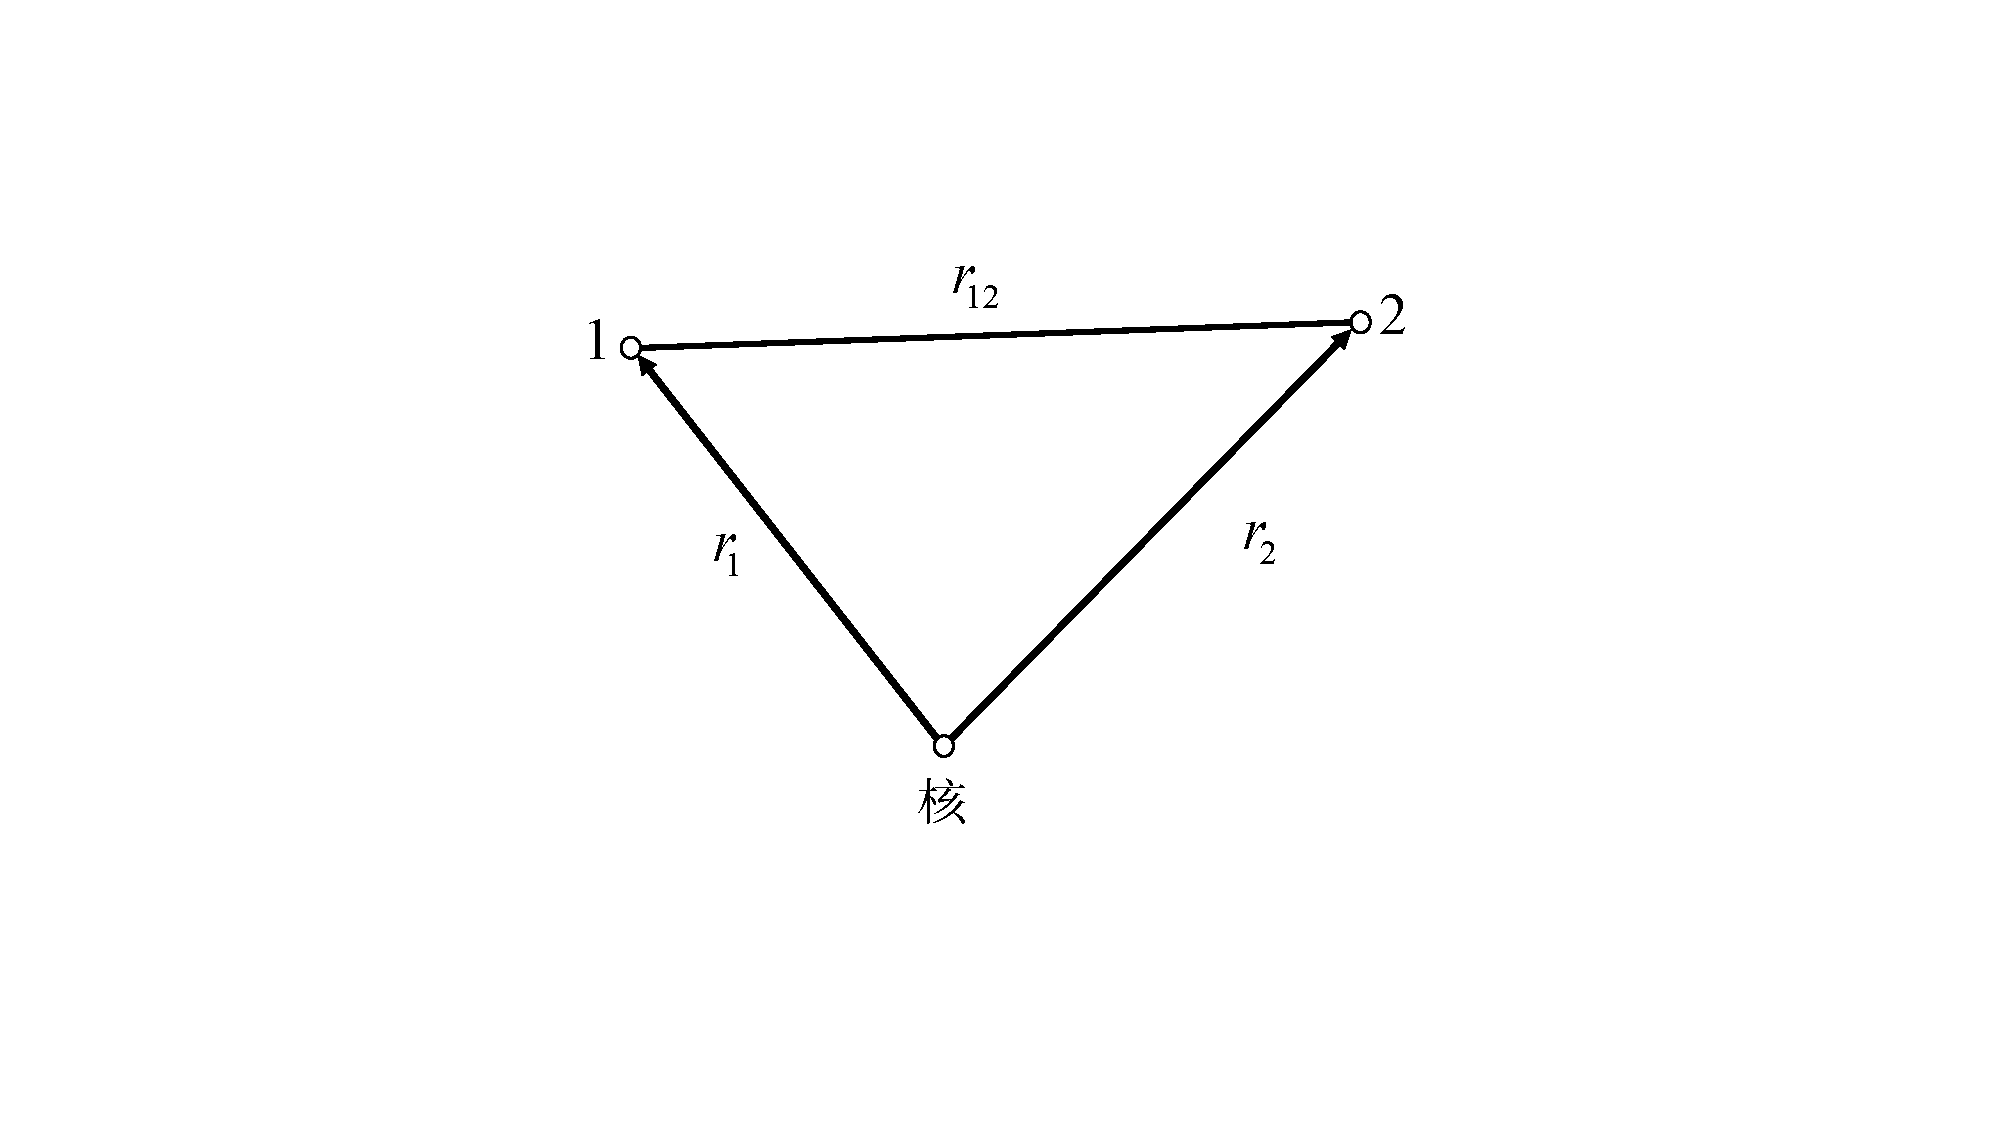
\includegraphics[width=3.5cm,clip]{QM file/figure/10-1}
	\caption{}\label{fig.10-1}
\end{wrapfigure}
这里略去了自旋-轨道耦合作用.


{\heiti 1. 正氦与仲氦}

体系的能级由定态薛定谔方程
\begin{empheq}{equation}\label{eqx3.2}
	H\Psi=E\Psi
\end{empheq}\eqllong
决定.由于$H$不含自旋变量,$\Psi$可以分离变量地表示成
\begin{equation}\label{eqx3.3}
	\Psi(q_{1},q_{2})=\varPsi(\boldsymbol{r}_{1},\boldsymbol{r}_{2})\chi(S_{1z},S_{2z})
\end{equation}\eqnormal
$\varPsi$为“轨道”波函数,$\chi$为自旋波函数.显然,$\varPsi$应该是$H$的本征函数,而$\chi$则与能级没有直接关系.

作为全同费密子体系的波函数,$\Psi$应该具有交换反对称性,即
\begin{empheq}{equation*}
	\hat{P}_{12}\Psi=(\hat{P}_{12}\varPsi)(\hat{P}_{12}\chi)=-\Psi=-\varPsi\chi
\end{empheq}\eqindent{1}
有两种可能的配合:
\begin{empheq}{align}
&(\si{i})	&&\hat{P}_{12}\varPsi=-\varPsi,\qquad \hat{P}_{12}\chi=\chi	\label{eqx3.4}\\
&(\si{ii})	&&\hat{P}_{12}\varPsi=\varPsi,\qquad \hat{P}_{12}\chi=-\chi	\label{eqx3.5}
\end{empheq}\eqnormal
第一种情形轨道波函数$\varPsi$是交换反对称的,自旋波函数则是交换对称的.第二种情形刚好相反.

二电子体系的自旋波函数共有4种(参看$\S$\ref{sec:07.08}),交换对称态有3种,即$\chi_{11},\chi_{10},\chi_{1-1}$,反对称态只有1种,即$\chi_{00}$.对称态相应于总自旋$S=1$,反对称态相应于$S=0$通常将氦原子按其自旋状态分类,称为正氦和仲氦:

正氦:$S=1,\chi=\chi_{11},\chi_{10},\chi_{1-1},\varPsi(\boldsymbol{r}_{1},\boldsymbol{r}_{2})$反对称

仲氦:$S=0,\chi=\chi_{00},\varPsi(\boldsymbol{r}_{1},\boldsymbol{r}_{2})$对称

\noindent 从表面上看,能级仅与$\varPsi(\boldsymbol{r}_{1},\boldsymbol{r}_{2})$有关,与$\chi$无直接关系.但因$\varPsi,\chi$的交换对称性互相制约,而$\varPsi$的交换对称性直接影响到体系的能量.[如$\varPsi$为反对称,$\varPsi(\boldsymbol{r}_{1},\boldsymbol{r}_{2})=-\varPsi(\boldsymbol{r}_{2},\boldsymbol{r}_{1})$,当$\boldsymbol{r}_{1}=\boldsymbol{r}_{2}$,$\varPsi=0$,因此两电子位置接近的概率较小,从而$\frac{\e^{2}}{r_{12}}$的平均值偏小.如$\varPsi$为交换对称,就没有这种性质.]所以正氦与仲氦将具有不同的能级.正氦的每一个能级都相应于自旋三重态,仲氦能级相应于自旋单态.

{\heiti 2. 微扰论} 

将两电子的相互作用势$\frac{\e^{2}}{r_{12}}$当作微扰,\eqref{eqx3.1}式可以表示成
\begin{empheq}{equation}\label{eqx3.6}
	H=H_{0}(\boldsymbol{r}_{1})+H_{0}(\boldsymbol{r}_{2})+H^{\prime}
\end{empheq}\eqlong
其中
\begin{empheq}{equation}\label{eqx3.7}
	H^{\prime}=\frac{\e^{2}}{r_{12}},\quad H_{0}(\boldsymbol{r}_{i})=-\frac{\hbar^{2}}{2m_{e}}\nabla_{i}^{2}-\frac{2\e^{2}}{r_{i}}\quad(i=1,2)
\end{empheq}\eqnormal
$H_{0}(\boldsymbol{r}_{i})$的本征值与本征函数就是类氢离子$(Z=2)$的能级与波函数
\begin{empheq}{equation}\label{eqx3.8}
	E_{n}=-\frac{4\e^{2}}{2n^{2}a_{0}},\quad \varPsi_{nlm}=R_{nl}Y_{lm}
\end{empheq}\eqlong
按照微扰论,轨道波函数的零级近似应该是$H_{0}(\boldsymbol{r}_{1})+H_{0}(\boldsymbol{r}_{2})$的本征函数,其一般形式为
\begin{empheq}{equation}\label{eqx3.9}
	\varPsi_{nlm}(\boldsymbol{r}_{1})\varPsi_{n^{\prime}l^{\prime}m^{\prime}}(\boldsymbol{r_{2}}),\quad \varPsi_{n^{\prime}l^{\prime}m^{\prime}}(\boldsymbol{r}_{1})\varPsi_{nlm}(\boldsymbol{r}_{2})
\end{empheq}\eqlllong
相应于能级(零级近似)$E_{n}+E_{n^{\prime}}$.在以下的叙述中,量子数$nlm$将简记成$n$.作为二电子体系的轨道波函数,应该具有交换对称或反对称性,显然应取下列形式:
\begin{empheq}{equation}\label{eqx3.10}
	\begin{aligned}
		\varPsi_{nn}^{S}(\boldsymbol{r}_{1},\boldsymbol{r}_{2}) &=\varPsi_{n}(\boldsymbol{r}_{1})\varPsi_{n}(\boldsymbol{r}_{2})	\\
		\varPsi_{nn^{\prime}}^{S}(\boldsymbol{r}_{1},\boldsymbol{r}_{2})	 &=\frac{1}{\sqrt{2}}[\varPsi_{n}(\boldsymbol{r}_{1})\varPsi_{n^{\prime}}(\boldsymbol{r_{2}})+\varPsi_{n^{\prime}}(\boldsymbol{r}_{1})\varPsi_{n}(\boldsymbol{r}_{2})]\quad (n\neq n^{\prime})		\\
		\varPsi_{nn^{\prime}}^{A}(\boldsymbol{r}_{1},\boldsymbol{r}_{2}) &=\frac{1}{\sqrt{2}}[\varPsi_{n}(\boldsymbol{r}_{1})\varPsi_{n^{\prime}}(\boldsymbol{r_{2}})-\varPsi_{n^{\prime}}(\boldsymbol{r}_{1})\varPsi_{n}(\boldsymbol{r}_{2})]\quad (n\neq n^{\prime})
	\end{aligned}
\end{empheq}\eqlong
由于微扰$H^{\prime}=\frac{\e^{2}}{r_{12}}$是交换对称的,必然有
\begin{empheq}{equation}\label{eqx3.11}
	\langle \varPsi^{S}|H^{\prime}|\varPsi^{A}\rangle=\iint\varPsi^{S*}\frac{\e^{2}}{r_{12}}\varPsi^{A}d\tau_{1}d\tau_{2}=0
\end{empheq}\eqnormal
(在上式中交换$\boldsymbol{r}_{1},\boldsymbol{r}_{2}$,相当于$\boldsymbol{r}_{1}$改写成$\boldsymbol{r}_{2}$,$\boldsymbol{r}_{2}$改写成$\boldsymbol{r}_{1}$,对于积分值显然没有影响.但这样做时,$\varPsi^{S}$,$\frac{\e^{2}}{r_{12}}$不变,$\varPsi^{A}$则要变号,因此积分值要变号.由此可知积分值必为.)按照简并化微扰论,既然微扰$H^{\prime}$并不造成对称态与反对称态间的耦合,能级的一级修正就等于$H^{\prime}$的平均值,记为
\begin{empheq}{equation}\label{eqx3.12}
	\begin{aligned}
		E_{nn}^{S} &= \langle \varPsi_{nn}^{S}|\frac{\e^{2}}{r_{12}}|\varPsi_{nn}^{S} \rangle 	\\
		E_{nn^{\prime}}^{S} &= \langle \varPsi_{nn^{\prime}}^{S}|\frac{\e^{2}}{r_{12}}|\varPsi_{nn^{\prime}}^{S} \rangle 	\\
		E_{nn^{\prime}}^{A} &= \langle \varPsi_{nn^{\prime}}^{S}|\frac{\e^{2}}{r_{12}}|\varPsi_{nn^{\prime}}^{A} \rangle 	
	\end{aligned}
\end{empheq}
显然
\begin{empheq}{align}\label{eqx3.13}
	E_{nn}^{S} &=\iint\frac{\e^{2}}{r_{12}}|\varPsi_{n}(\boldsymbol{r}_{1})|^{2}|\varPsi_{n}(\boldsymbol{r}_{2})|^{2}d\tau_{1}d\tau_{2}	\nonumber\\
	&\equiv C(n,n)
\end{empheq}
这是电子1,2均处于轨道态$\varPsi_{n}$时,它们之间的库仑作用势的平均值.对于\eqref{eqx3.12}式的后二式,可以算出
\begin{empheq}{align}
	E_{nn^{\prime}}^{S} &=C(n,n^{\prime})+J(n,n^{\prime})	\label{eqx3.14}\\
	E_{nn^{\prime}}^{A} &=C(n,n^{\prime})-J(n,n^{\prime})	\label{eqx3.15}
\end{empheq}\eqlong
其中
\begin{empheq}{align}
	C(n,n^{\prime}) &=\iint\frac{\e^{2}}{r_{12}}|\varPsi_{n}(\boldsymbol{r}_{1})|^{2}|\varPsi_{n^{\prime}}(\boldsymbol{r}_{2})|^{2}d\tau_{1}d\tau_{2}	\nonumber\\
	&=\iint\frac{\e^{2}}{r_{12}}|\varPsi_{n^{\prime}}(\boldsymbol{r}_{1})|^{2}|\varPsi_{n}(\boldsymbol{r}_{2})|^{2}d\tau_{1}d\tau_{2}		\label{eqx3.16}\\
	J(n,n^{\prime}) &=\iint\frac{\e^{2}}{r_{12}}\varPsi_{n}^{*}(\boldsymbol{r}_{1})\varPsi_{n^{\prime}}(\boldsymbol{r}_{1})\varPsi_{n^{\prime}}^{*}(\boldsymbol{r}_{2})\varPsi_{n}(\boldsymbol{r}_{2})d\tau_{1}d\tau_{2}	\label{eqx3.17}
\end{empheq}
习惯上称$C(n,n^{\prime})$为“库仑能”,称$J(n,n^{\prime})$为“交换能”,其实它们都是两电子间库仑作用势$\frac{\e^{2}}{r_{12}}$平均值的一部分.从形式上看,$C(n,n^{\prime})$相当于一个电子处于$\varPsi_{n}$态,另一个电子处于$\varPsi_{n^{\prime}}$态时$\frac{\e^{2}}{r_{12}}$的平均值.$J(n,n^{\prime})$则没有这样直观简单的解释,它是两个电子交换其单电子态的产物,根源在于波函数的交换对称性.

总结上述计算,准确到微扰论一级近似,氦原子能级为:

正氦($S=1$,$\varPsi$反对称)
\begin{empheq}{equation}\label{eqx3.18}
	E=E_{n}+E_{n^{\prime}}+C(n,n^{\prime})-J(n,n^{\prime})\quad (n\neq n^{\prime})
\end{empheq}

仲氦($S=0$,$\varPsi$对称)
\begin{empheq}{align}
	E&=2E_{n}+C(n,n)\quad (n=n^{\prime})		\label{eqx3.19}\\
	E&=E_{n}+E_{n^{\prime}}+C(n,n^{\prime})+J(n,n^{\prime})\quad (n\neq n^{\prime})	\label{eqx3.20}
\end{empheq}\eqnormal
$C(n,n^{\prime})$与$J(n,n^{\prime})$的计算相当繁,从略.当$n,n^{\prime}$较小时,$C$与$J$均为正,但$J(n,n^{\prime})<C(n,n^{\prime})$,所以当$n\neq n^{\prime}$,正氦和仲氦能级接近,仲氦稍高.但仲氦还有$n=n^{\prime}$(两个电子处于相同状态)的能级,即\eqref{eqx3.19}式.氦原子的低激发态,一个电子处于最低的$E_{1}$能级($\varPsi_{100}$态),另一个电子处于$E_{n}$能级($\varPsi_{nlm}$态,$n\geqslant2$),由于$\varPsi_{100}$与$\varPsi_{nlm}$重叠较少,因此交换能$J(100,nlm)$显得微不足道.只有当两个电子同处一个壳层($n$相同,$lm\neq l^{\prime}m^{\prime}$),空间位置较接近,交换能才变得重要.

{\heiti 3. 基态(微扰论及变分法)} 

氦原子的基态属于仲氦,两个电子同处轨道态$\varPsi_{100}$,总自旋为0.按照微扰论,轨道波函数(零级近似)为
\begin{empheq}{equation}\label{eqx3.21}
	\varPsi_{100,100}^{S}(r_{1},r_{2})=\varPsi_{100}(r_{1})\varPsi_{100}(r_{2})
\end{empheq}
其中$\varPsi_{100}$为类氢离子$(Z=2)$基态波函数,即
\begin{empheq}{equation}\label{eqx3.22}
	\varPsi_{100}(r)=\left(\frac{8}{\pi a_{0}^{3}}\right)^{\frac{1}{2}}e^{-2r/a_{0}}
\end{empheq}
利用公式
\begin{empheq}{equation}\label{eqx3.23}
	\iint\frac{1}{r_{12}}e^{-\alpha(r_{1}+r_{2})}d\tau_{1}d\tau_{2}=\frac{20\pi^{2}}{\alpha^{5}}\quad (\alpha>0)
\end{empheq}
(证明见本节末)容易算出
\begin{empheq}{equation}\label{eqx3.24}
	C(100,100)=\frac{5}{4}\cdot\frac{\e^{2}}{a_{0}}
\end{empheq}\eqlong
因此氦原子基态能量的微扰论结果为
\begin{empheq}{equation}\label{eqx3.25}
	E_{0}(\text{微扰论})=2E_{1}+C(100,100)=-\num{2.75}\frac{\e^{2}}{a_{0}}
\end{empheq}\eqnormal
实验值则是
\begin{empheq}{equation*}
	E_{0}(\text{实验})=-\num{79.01}\si{eV}=-\num{2.9037}\frac{\e^{2}}{a_{0}}
\end{empheq}
二者约相差5.3\%.

在上述微扰论计算中,电子的轨道波函数\eqref{eqx3.22}式描述的是电子在原子核所生库仑场中的运动,忽略了另一个电子的存在所产生的影明.事实上,另一个电子的存在,将在一定程度上对核电荷起屏蔽作用,每一个电子感受到的总库仑势(原子核及另一个电子的库仑势之和)粗略地等效于电荷$\lambda e(1<\lambda<2)$产生的库仑势如改用变分法计算,就可以反映这种屏蔽效应.取变分试探函数
\begin{empheq}{align}\label{eqx3.26}
	\varPsi(\lambda,r_{1},r_{2}) &=\varPsi(\lambda,r_{1})\varPsi(\lambda,r_{2})	\nonumber\\
	&=\frac{\lambda^{3}}{\pi a_{0}^{3}}e^{-\lambda r_{1}/a_{0}}e^{-\lambda r_{2}/a_{0}}
\end{empheq}
作为氦原子基态轨道波函数的近似,其中$\lambda$为变分参数.上式已经归一化.当$\lambda=2$,上式就是\eqref{eqx3.21}式.

对\eqref{eqx3.26}式计算总能量H的平均值,即
\begin{empheq}{equation*}
	E(\lambda)=\langle\varPsi(\lambda,r_{1},r_{2})|H|\varPsi(\lambda,r_{1},r_{2})\rangle 
\end{empheq}\eqlong
容易求得
\begin{empheq}{align}
	\langle\nabla_{1}^{2}\rangle =&\langle\nabla_{2}^{2}\rangle=\int\varPsi(\lambda,r)\nabla^{2}\varPsi(\lambda,r)d\tau	\nonumber\\
	=&-\int|\nabla\varPsi(\lambda,r)|^{2}d\tau=-\left(\frac{\lambda}{a_{0}}\right)-\nonumber \\
	&\frac{\hbar^{2}}{2m_{e}}\langle\nabla_{1}^{2}+\nabla_{2}^{2}\rangle=\frac{\hbar^{2}\lambda^{2}}{m_{e}a_{0}}=\lambda^{2}\frac{\e^{2}}{a_{0}} \label{eqx3.27}\\
	\left\langle\frac{1}{r_{1}}\right\rangle=&\left\langle\frac{1}{r_{2}}\right\rangle=\int\frac{1}{r}\varPsi^{2}(\lambda,r)d\tau=\frac{\lambda}{a_{0}}-\nonumber\\& 2\e^{2}\left\langle\frac{1}{r_{1}}+\frac{1}{r_{2}}\right\rangle=-4\lambda\frac{\e^{2}}{a_{0}}		\label{eqx3.28}\\
	\left\langle\frac{\e^{2}}{r_{12}}\right\rangle=&\e^{2}\iint\frac{1}{r_{12}}\varPsi^{2}(\lambda,r_{1})\varPsi^{2}(\lambda,r_{2})d\tau_{1}d\tau_{2}	\nonumber\\
	=&\frac{5\lambda}{8}\frac{\e^{2}}{a_{0}}		\label{eqx3.29}
\end{empheq}\eqnormal
因此
\begin{empheq}{equation}\label{eqx3.30}
	E(\lambda)=\left(\lambda^{2}-\frac{27}{8}\lambda\right)\frac{\e^{2}}{a_{0}}
\end{empheq}
由极值条件$\frac{\partial E(\lambda)}{\partial\lambda}$.求得$\lambda$的最佳值为$\lambda_{0}=\frac{27}{16}$.所以基态能级的变分法结果为
\begin{empheq}{equation}\label{eqx3.31}
	E(\lambda_{0})=-\left(\frac{27}{16}\right)^{2}\frac{\e^{2}}{a_{0}}=-\num{2.8477}\frac{\e^{2}}{a_{0}}
\end{empheq}
这结果比实验值略高,二者相差1.93\%.与微扰论结果相比,变分法结果已大有改进.如果试探波函数的构造再复杂一些,结果还可以改善,直到与实验值完全符合.由此可见,量子力学理论辅以恰当的数学方法,可以成功地处理原子构造问题.

\eqref{eqx3.23}式的证明如下.将积分写成
\begin{empheq}{equation*}
	I-\iint d\tau_{2}I_{1}e^{-\alpha r_{2}},\quad I_{1}=\int\frac{1}{r_{12}}e^{-\alpha r_{1}}d\tau_{1}
\end{empheq}
计算$I_{1}$时,取$\boldsymbol{r}_{2}$为极轴(参看图\ref{fig.10-2}),$\boldsymbol{r}_{1}$用球坐标,则
\begin{empheq}{align*}
	d\tau_{1}&=r_{1}^{2}dr_{1}\sin\theta d\theta d\varphi	\\
	r_{12}&=(r_{1}^{2}+r_{2}^{2}-2r_{1}r_{2}\cos\theta)^{\frac{1}{2}}
\end{empheq}\eqindent{3}
\begin{wrapfigure}[6]{r}{5em}
	\centering
	\small
	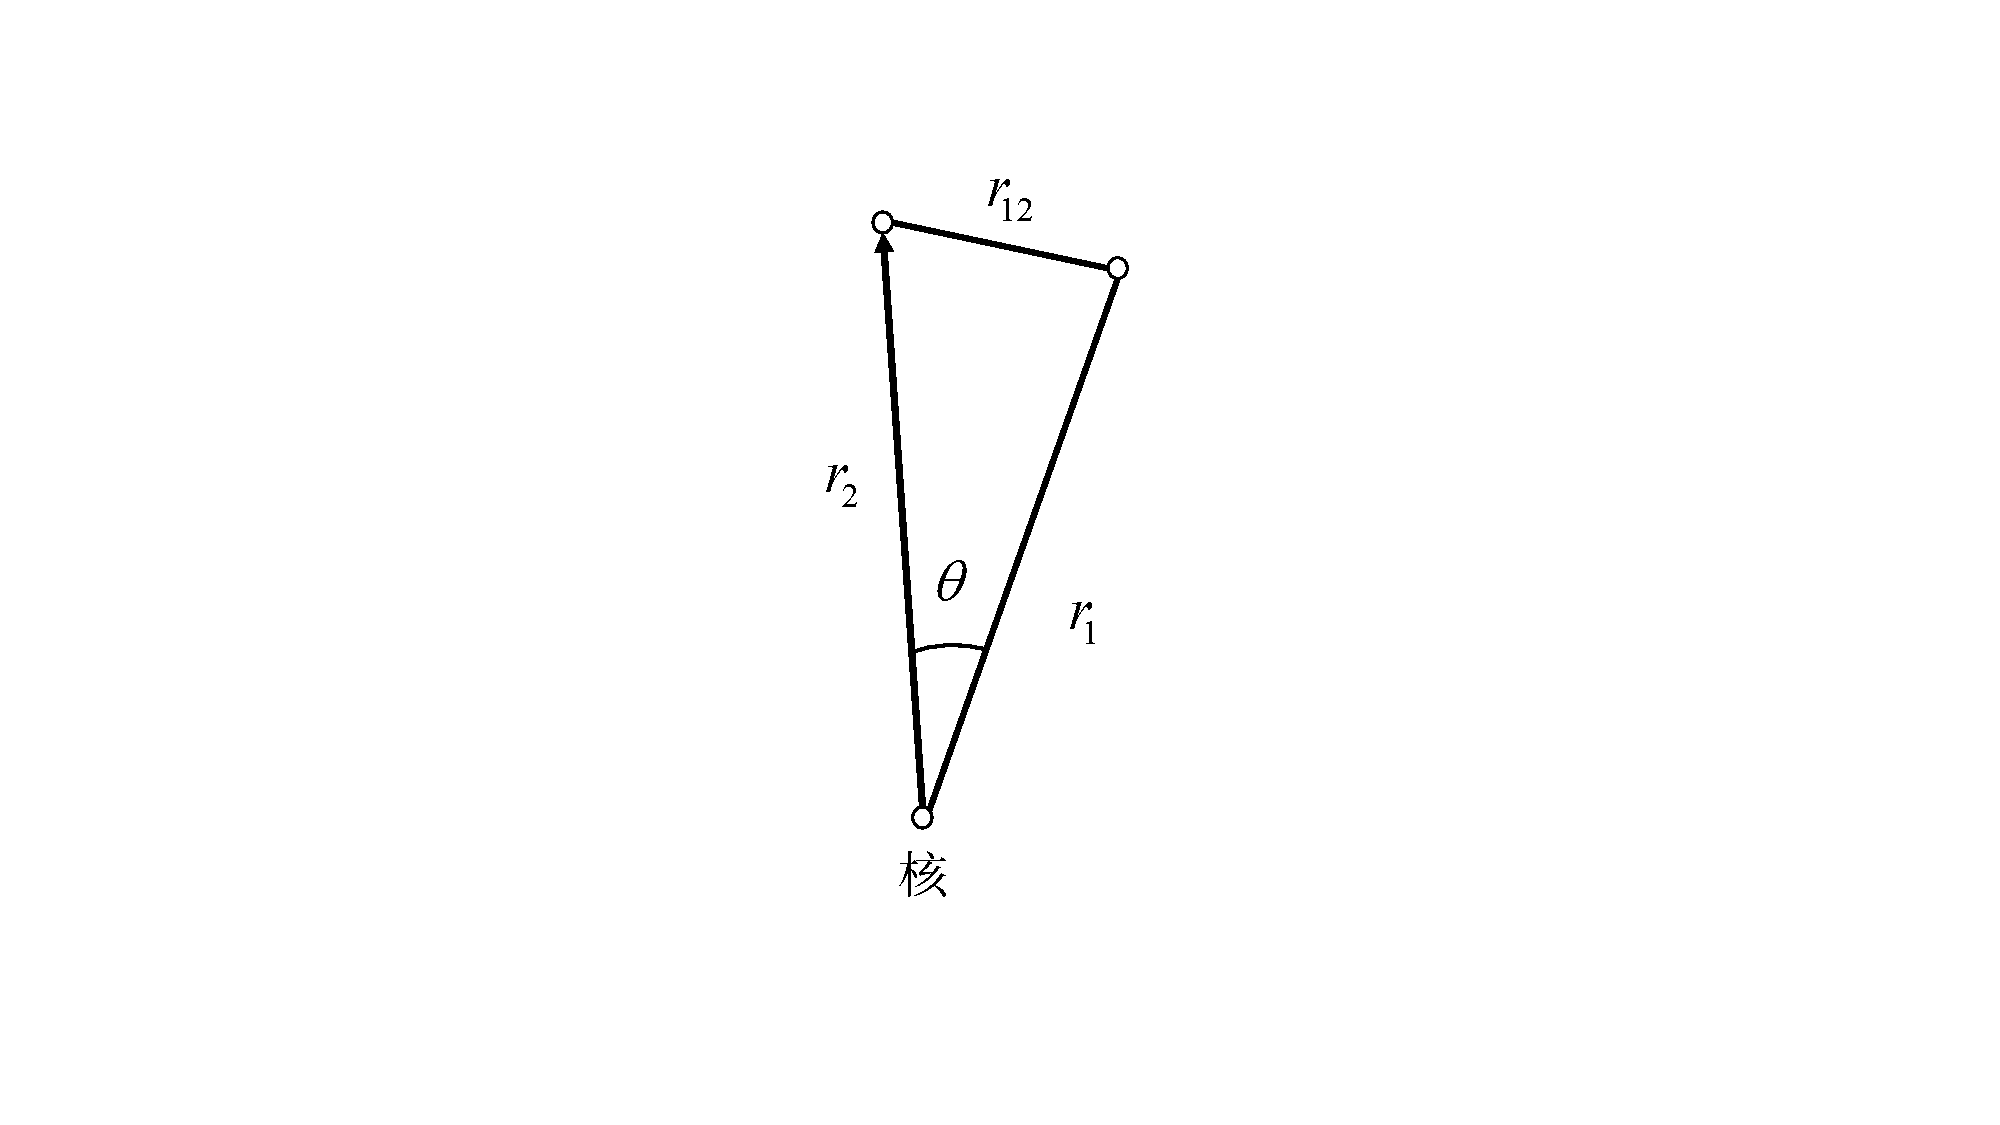
\includegraphics[width=2cm,clip]{QM file/figure/10-2}
	\caption{}\label{fig.10-2}
\end{wrapfigure}
容易算出
\begin{empheq}{equation*}
	I_{1}=\int_{0}^{\infty}dr_{1}r_{1}^{2}e^{-\alpha r_{1}}2\pi\int_{0}^{\pi}(r_{1}^{2}+r_{2}^{2}-2r_{1}r_{2}\cos\theta)^{\frac{1}{2}}\sin\theta d\theta
\end{empheq}\eqlong
其中
\begin{empheq}{align*}
	&\int_{0}^{\pi}(r_{1}^{2}+r_{2}^{2}-2r_{1}r_{2}\cos\theta)^{\frac{1}{2}}\sin\theta d\theta	\\
	=&\frac{1}{r_{1}r_{2}}(r_{1}^{2}+r_{2}^{2}-2r_{1}r_{2}\cos\theta)^{\frac{1}{2}}\bigg|_{\theta=0}^{\theta=\pi} \\
	=&\frac{1}{r_{1}r_{2}}[(r_{1}+r_{2})-|r_{1}-r_{2}|]	\\
	=&\begin{dcases}
		\frac{2}{r_{2}},\quad r_{1}<r_{2}	\\
		\frac{2}{r_{1}},\quad r_{1}>r_{2}
	\end{dcases}	
\end{empheq}
因此
\begin{empheq}{align*}
	I_{1}=&4\pi\int_{0}^{r_{2}}\frac{1}{r_{2}}r_{1}^{2}e^{-\alpha r_{1}}dr_{1}+4\pi\int_{r_{2}}^{\infty}r_{1}e^{-\alpha r_{1}}dr_{1}	\\
	&=\frac{4\pi}{\alpha^{2}}\left[ \frac{2}{\alpha r_{2}}-\left(1+\frac{2}{\alpha r_{2}}\right)e^{-\alpha r_{2}} \right]
\end{empheq}
代入$I$中,即得
\begin{empheq}{align*}
	I&=r\pi\int_{0}^{\infty}I_{1}e^{-\alpha r_{2}}r_{2}^{2}dr_{2}	\\
	&=\frac{16\pi^{2}}{\alpha^{5}}\int_{0}^{\infty}x^{2}e^{-x}\left[\frac{2}{x}-\left(1+\frac{2}{x}\right)e^{-x} \right]	\\
	&=20\pi^{2}/\alpha^{5}
\end{empheq}\eqnormal
此即\eqref{eqx3.23}式.





% 氢分子
\section[氢分子]{氢分子} \label{sec:10.04} % 
% \makebox[5em][s]{} % 短题目拉间距

1927年,Heitler-London用量子力学方法研究氢分子结构获得成功,开创了量子化学.

氢分子包含两个原子核$(a,b)$及两个电子$(1,2)$,如图\ref{fig.10-3} 所示.如略去原子核的运动(即分子的振动、转动和平移),就可以将氢分子当作二电子体系,体系的总能量算符可以表示成
\eqllong
\begin{empheq}{align}\label{eqx4.1}
	H=&-\frac{\hbar^{2}}{2m_{e}}(\nabla_{1}^{2}+\nabla_{2}^{2})-\e^{2}(\frac{1}{r_{1a}}+\frac{1}{r_{1b}}+\frac{1}{r_{2a}}+\frac{1}{r_{2b}})+ \nonumber\\
	&\frac{\e^{2}}{r_{12}}+\frac{\e^{2}}{R}
\end{empheq}
\begin{wrapfigure}[7]{r}{8em}
	\centering
	\small
	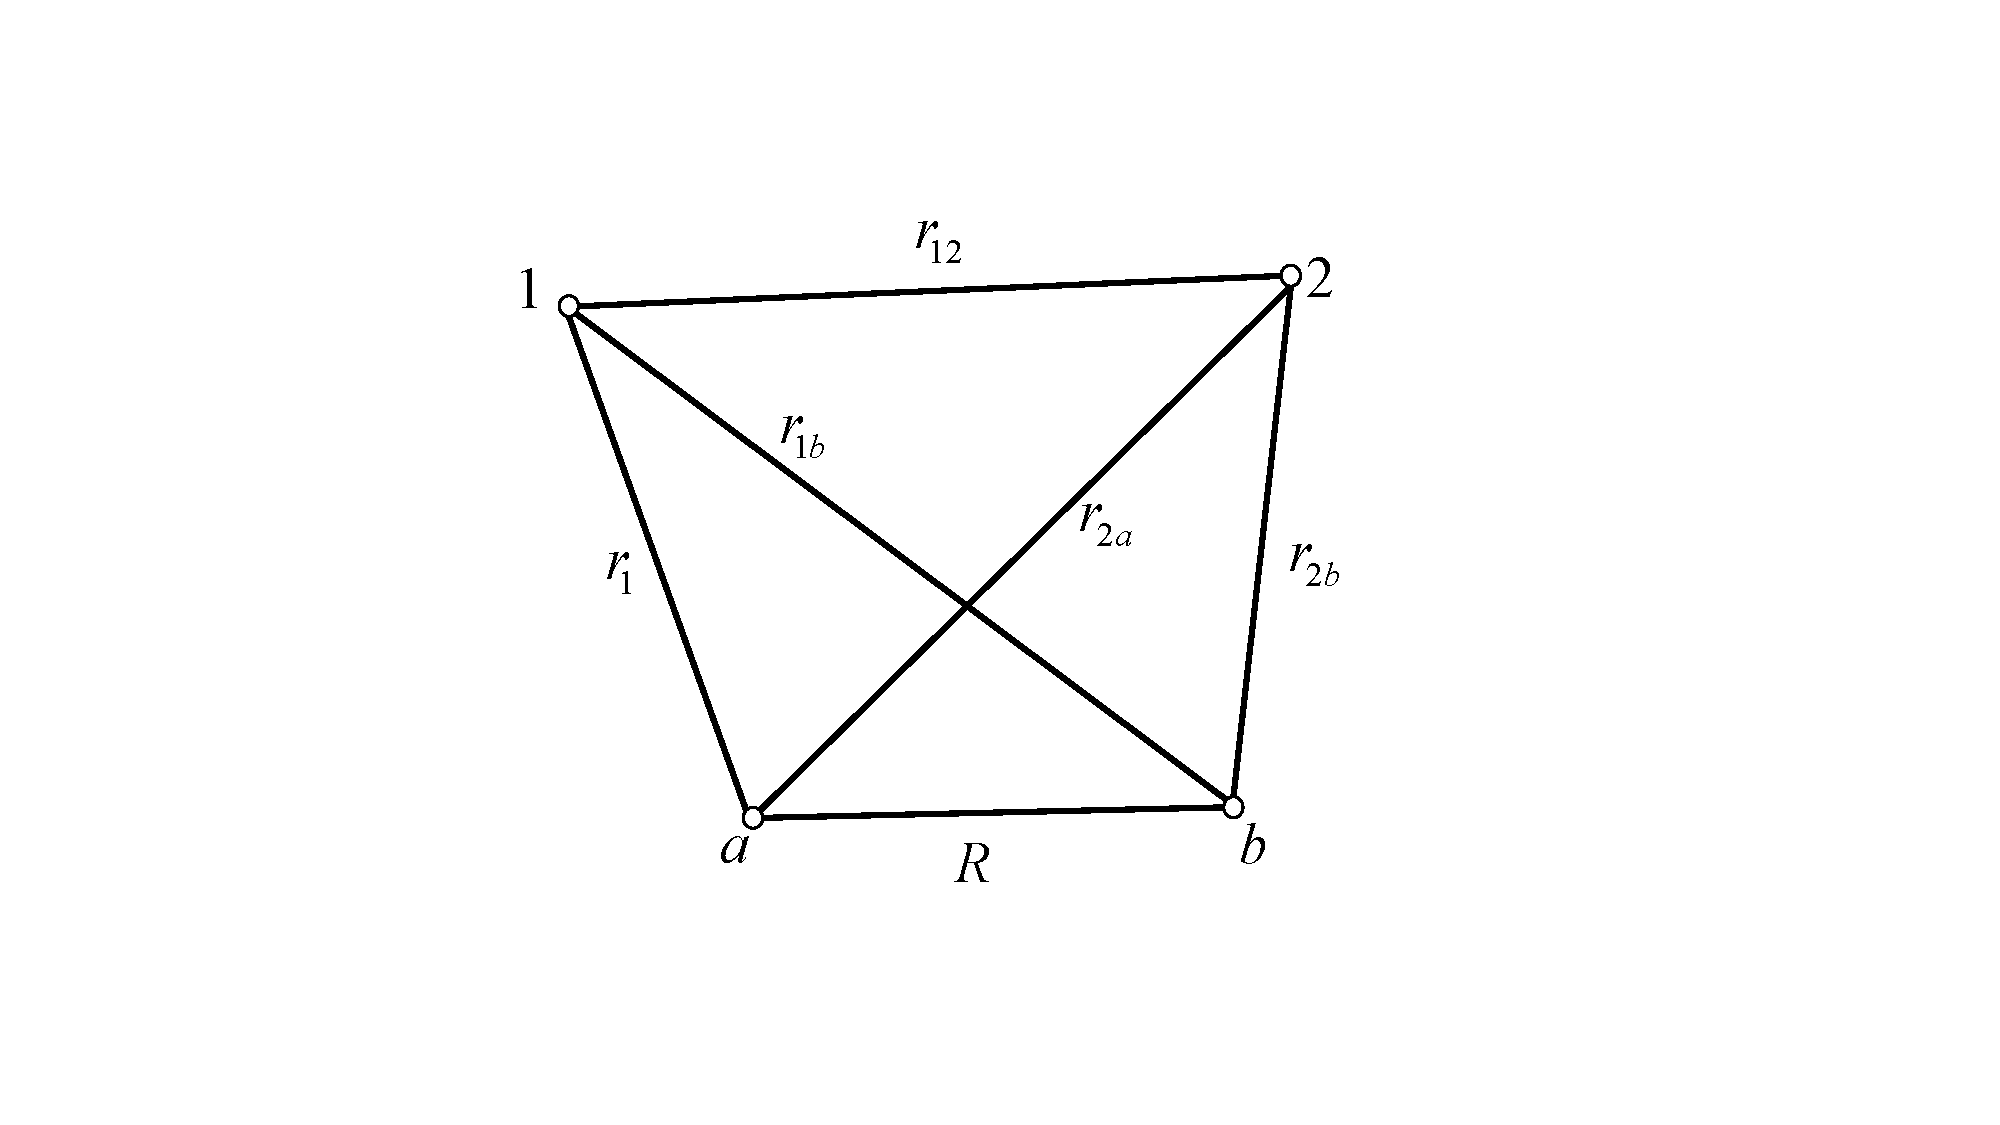
\includegraphics[width=3cm,clip]{QM file/figure/10-3}
	\caption{}\label{fig.10-3}
\end{wrapfigure}
其中共包含6项库仑作用势,最后一项是原子核$a,b$间的库仑能,它是分子能量的一部分,所以应包含在$H$中.在计算中$R$作为参量处理.

和氦原子相仿,二电子体系总波函数可以表示成轨道波函数与自旋波函数的积,
\begin{empheq}{equation}\label{eqx4.2}
	\Psi(q_{1},q_{2})=\varPsi(\boldsymbol{r}_{1},\boldsymbol{r}_{2})\chi(S_{1z},S_{2z})
\end{empheq}\eqnormal
$\varPsi$应满足能量本征方程
\begin{empheq}{equation}\label{eqx4.3}
	H\varPsi(\boldsymbol{r}_{1},\boldsymbol{r}_{2})=E\varPsi(\boldsymbol{r}_{1},\boldsymbol{r}_{2})
\end{empheq}
关于$\varPsi$及$\chi$的交换对称性的讨论以及结论,和氦原子相同,不再重述.由于有两个原子核(即两个库仑力中心),数学处理显然比氦原子更为困难.近似方法通常与物理模型结合使用,大致可分两类,即分子轨函法和原子轨函法.所谓分子轨道是指在原子核$a,b$的库仑场的共同作用下形成的单电子状态,也就是氢分子离子$(\ce{H_{2}^{+}})$的电子轨道态.氢分子的两个电子都处于分子轨道的基态.(自旋态$\chi_{00},S=0$电子间库仑作用$\frac{\e^{2}}{r_{12}}$则作为微扰处理.至于分子轨道波函数的确定仍然要用近似方法(两个库仑力中心!)所谓原子轨道是指孤立原子的单电子状态$\varPsi_{nlm}$.以此作为基础,设法计算两个原子的相互作用能.Heitler-London方法就是原子轨函法,这种方法计算方便,但是精确程度不如分子轨函法.本节只介绍原子轨函法.

考虑分子的形成过程如下:两个孤立的原子逐渐靠近,由于相互作用(电荷间的库仑作用)而结合成分子.以两个原子波函数的积作为分子波函数的零级近似,两原子的相互作用当作微扰.电子与原子核的配对有两种可能,(以每个原子核拥有一个电子为前提,相当于共价键;如二电子同属于一个原子核,就形成离子键.氢分子基本上是共价键类型)如图\ref{fig.10-4}所示,图左相当于原子$(a,2)$与$(b,1)$结合成分子,图右相当于原子$(a,2)$与$(b,1)$结合成分子,两种情形的轨道波函数分别为
\begin{figure}[!h]
	\centering
	\small
	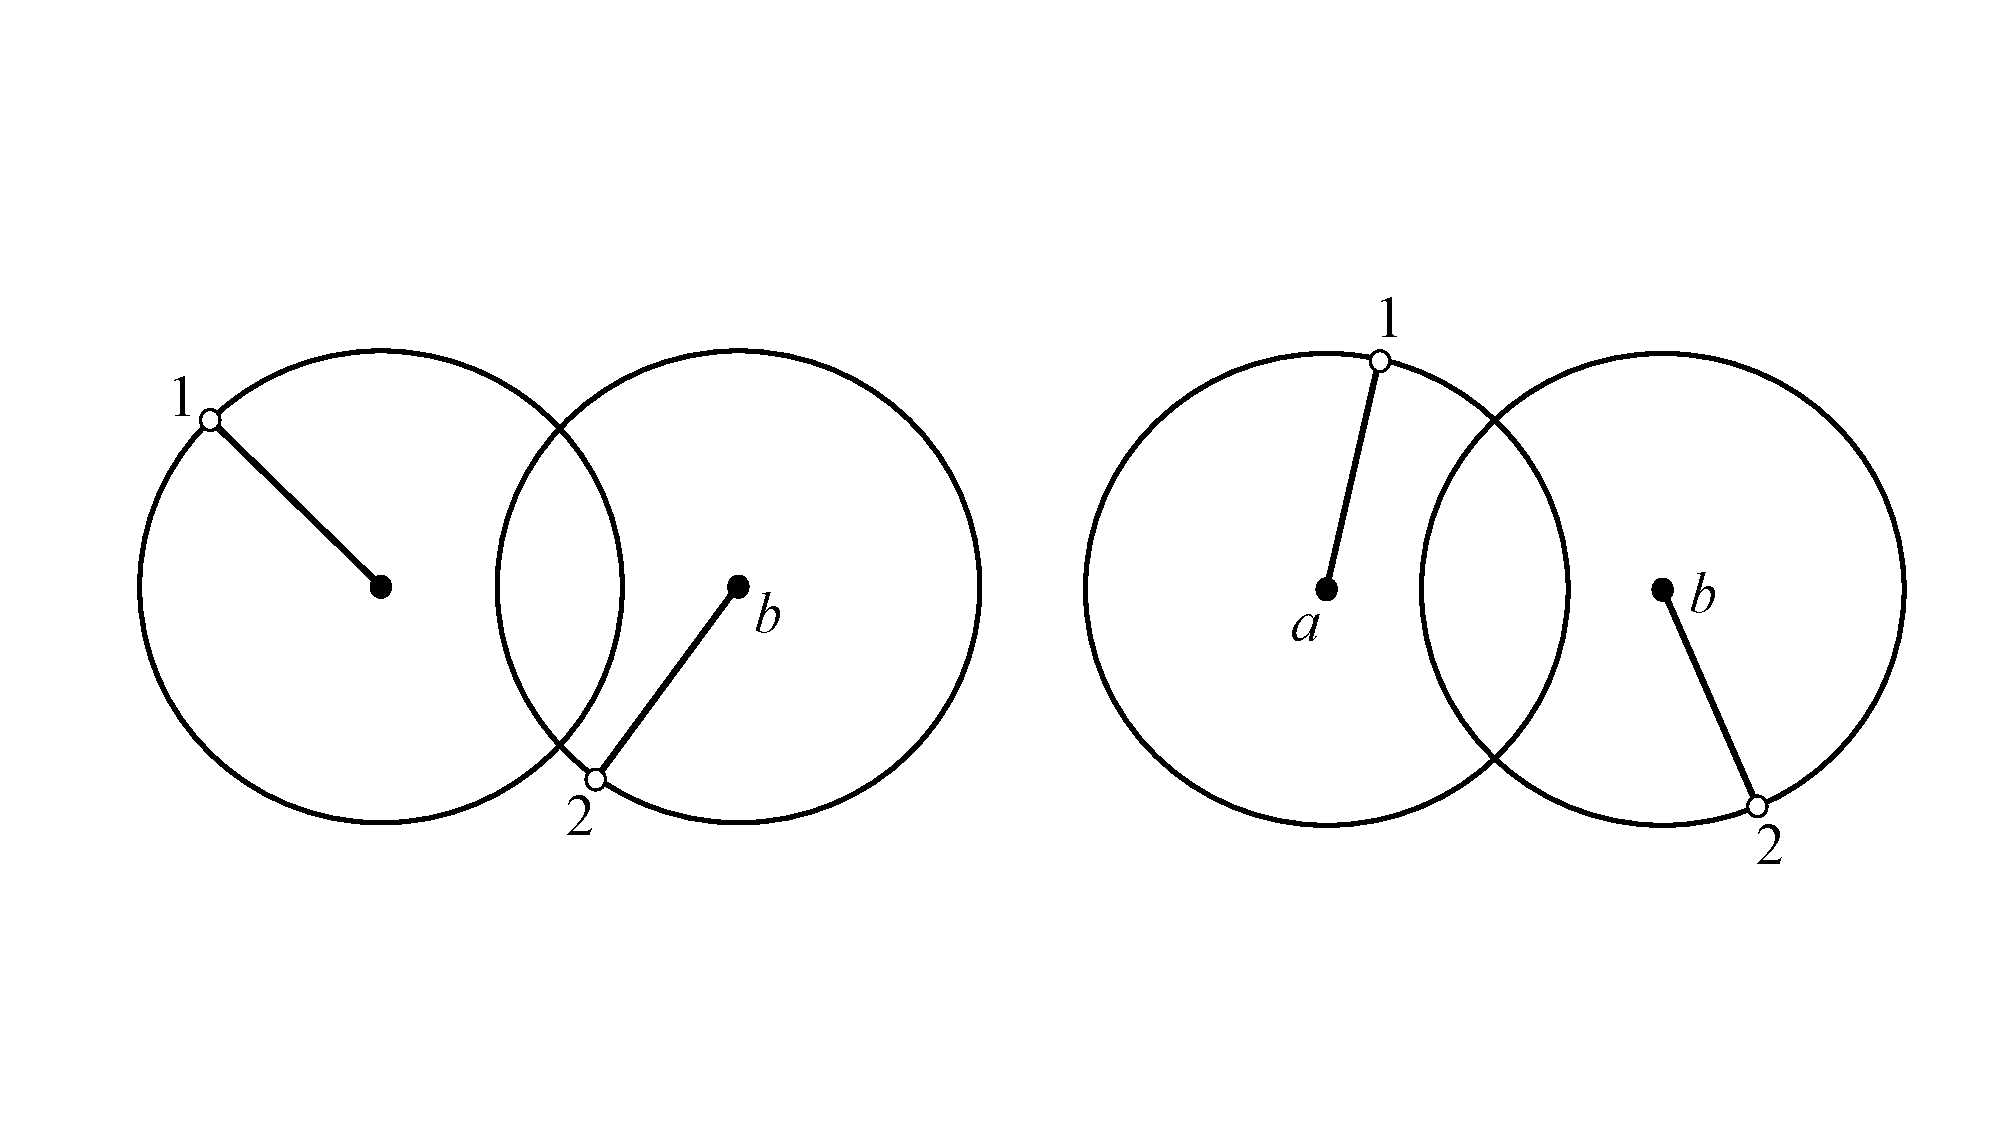
\includegraphics[width=7cm,clip]{QM file/figure/10-4}
	\caption{}\label{fig.10-4}
\end{figure}
\begin{empheq}{equation}\label{eqx4.4}
	\varPsi_{a}(1)\varPsi_{b}(2),\quad \varPsi_{a}(2)\varPsi_{b}(1)
\end{empheq}
其中$\varPsi_{a}(1)$指氢原子$(a,1)$的基态波函数,即
\begin{empheq}{equation}\label{eqx4.5}
	\varPsi_{a}(1)=\varPsi_{100}(r_{1a})=\left(\frac{1}{\pi a_{0}^{3}}\right)^{\frac{1}{2}}e^{-r_{1a}/a_{0}}
\end{empheq}
依此类推.将总能$H$分成$H_{0}$和$H^{\prime}$,$H_{0}$是与两个氢原子的构成有关的算符,$H^{\prime}$是两个原子的相互作用能.对于\eqref{eqx4.4}式中第一个波函数$\varPsi_{a}(1)\varPsi_{b}(2)$,$H_{0}$与$H^{\prime}$分别是
\begin{empheq}{equation}\label{eqx4.6}
	\begin{aligned}
		H_{0} &=-\frac{\hbar^{2}}{2m_{e}}(\nabla_{1}^{2}+\nabla_{2}^{2})-\frac{\e^{2}}{r_{1a}}-\frac{\e^{2}}{r_{1b}}	\\
		H^{\prime} &=\frac{\e^{2}}{R}+\frac{\e^{2}}{r_{12}}-\frac{\e^{2}}{r_{1b}}-\frac{\e^{2}}{r_{2a}}
	\end{aligned}
\end{empheq}
显然
\begin{empheq}{equation*}
	H_{0}\varPsi_{a}(1)\varPsi_{b}(2)=2E_{1}\varPsi_{a}(1)\varPsi_{b}(2),\quad E_{1}=-\frac{\e^{2}}{2a_{0}}
\end{empheq}
$E_{k}$是氢原子基态能级.对于\eqref{eqx4.4}式中第二个波函数$\varPsi_{a}(2)\varPsi_{a}(1)$,$H_{0}$与$H^{\prime}$应取
\begin{empheq}{equation*}\label{eqx4.6'}
	\begin{aligned}
		H_{0} &=-\frac{\hbar^{2}}{2m_{e}}(\nabla_{1}^{2}+\nabla_{2}^{2})-\frac{\e^{2}}{r_{1b}}-\frac{\e^{2}}{r_{2a}}	\\
		H^{\prime} &=\frac{\e^{2}}{R}+\frac{\e^{2}}{r_{12}}-\frac{\e^{2}}{r_{1a}}-\frac{\e^{2}}{r_{2b}}
	\end{aligned}\tag{$10.4.6^{\prime}$}
\end{empheq}
显然
\begin{empheq}{equation*}
	H_{0}\varPsi_{a}(2)\varPsi_{b}(1)=2E_{1}\varPsi_{a}(2)\varPsi_{b}(1)
\end{empheq}\eqlong

如果不管波函数的交换对称性,简单地以\eqref{eqx4.4}式中任何一个(例如第一个)波函数$\varPsi_{a}(1)\varPsi_{b}(2)$作为分子的近似波函数,而以$H^{\prime}$平均值当作分子的结合能,记为$W$,则
\begin{empheq}{equation}\label{eqx4.7}
	W=\iint\varPsi_{a}^{2}(1)\varPsi_{b}^{2}\left(\frac{\e^{2}}{R}+\frac{\e^{2}}{r_{12}}-\frac{\e^{2}}{r_{1b}}-\frac{\e^{2}}{r_{2a}}\right)e^{-2R/a_{0}}
\end{empheq}
$W$之值显然与$R$有关,计算结果为
\begin{empheq}{equation}\label{eqx4.8}
	W=\frac{\e^{2}}{a_{0}}\left(\frac{a_{0}}{R}+\frac{5}{8}-\frac{3}{4}\frac{R}{a_{0}}-\frac{1}{6}\frac{R^{2}}{a_{0}^{2}}\right)e^{-2R/a_{0}}
\end{empheq}
当$R=1.87 a_{0}$时$W$取极小值,
\begin{empheq}{equation}\label{eqx4.9}
	W(R=1.87 a_{0})=-\num{0.0196}\left(\frac{\e^{2}}{a_{0}}\right)=-\num{0.533}\si{eV}.
\end{empheq}\eqnormal
而氢分子结合能的实验值是\num{-4.72}\si{eV},键长$R=\num{0.07395}\si{nm}$.\eqref{eqx4.9}式与实验值相差太多,量级不符合,由此可见,如不考虑波函数的交换对称性,就不能解释氢分子的形成.

考虑到交换对称性,氢分子轨道波函数(零级近似)应取\eqref{eqx4.4}式中两项的对称或反对称组合.以$\varPsi_{ab}^{S}(\boldsymbol{r}_{1},\boldsymbol{r}_{2})$和$\varPsi_{ab}^{A}(\boldsymbol{r}_{1},\boldsymbol{r}_{2})$表示对称和反对称轨道波函数,它们是
\begin{empheq}{align}
	\varPsi_{ab}^{S} &=C_{S}[\varPsi_{a}(1)\varPsi_{b}(2)+\varPsi_{a}(2)\varPsi_{b}(1)]	\label{eqx4.10}\\
	\varPsi_{ab}^{A} &=C_{A}[\varPsi_{a}(1)\varPsi_{b}(2)-\varPsi_{a}(2)\varPsi_{b}(1)]	\label{eqx4.11}
\end{empheq}
$C_{S}$及$C_{A}$是归一化常数.由于叠加的两个波函数并不正交,$C_{S}$及$C_{A}$均不等于$\frac{1}{\sqrt{2}}$.原子轨道波函数$\varPsi_{a}(1)$等已经归一化.定义重叠积分
\begin{empheq}{align}\label{eqx4.12}
	D 	&=\int\varPsi_{a}(1)\varPsi_{b}(1)d\tau_{1}	\nonumber\\
		&=\frac{1}{\pi a_{0}^{3}}\int e^{-(r_{1a}+r_{1b})/a_{0}}d\tau_{1}	\nonumber\\
		&=\left(1+\frac{R}{a_{0}}+\frac{1}{3}\frac{R^{2}}{a_{0}^{2}}\right)e^{-R/a_{0}}
\end{empheq}
则
\begin{empheq}{equation}\label{eqx4.13}
	C_{S}^{2}=\frac{1}{2+2D^{2}},\quad C_{A}^{2}=\frac{1}{2-2D^{2}}
\end{empheq}
当$R\rightarrow0$,原子核$a,b$重合,$\varPsi_{a}=\varPsi_{b}$,$D\rightarrow1$.当$R\rightarrow\infty$,$\varPsi_{a}$与$\varPsi_{b}$完全不重叠,$D\rightarrow0$.用本节所述方法处理氢分子构造,所得键长$R=\num{0.08}\si{nm}=\num{1.518}a_{0},D=\num{0.72},D^{2}=\num{0.52}$.

对于\eqref{eqx4.10}、\eqref{eqx4.11}式分别计算$H^{\prime}$平均值,分别记为$V_{ab}^{S},V_{ab}^{A}$,则可算出
\begin{empheq}{align}
	V_{ab}^{S} &=\iint\varPsi_{ab}^{S}H^{\prime}\varPsi_{ab}^{S}d\tau_{1}d\tau_{2}	\nonumber\\
	&=\frac{W+J}{1+D^{2}}	\label{eqx4.14}\\
	V_{ab}^{A} &=\iint\varPsi_{ab}^{A}H^{\prime}\varPsi_{ab}^{A}d\tau_{1}d\tau_{2}	\nonumber\\
	&=\frac{W-J}{1-D^{2}}		\label{eqx4.15}
\end{empheq}\eqindent{1}
计算时$H^{\prime}$应视作用的对象而取\eqref{eqx4.6}式或\eqref{eqx4.6'}式.$W$由\eqref{eqx4.8}式表示,$J$由下式表示,
\begin{empheq}{align}\label{eqx4.16}
	J	&=\iint\varPsi_{a}(1)\varPsi_{b}(2)\left(\frac{\e^{2}}{R}+\frac{\e^{2}}{r_{12}}-\frac{\e^{2}}{r_{1a}}-\frac{\e^{2}}{r_{2b}}\right)\varPsi_{a}(2)\varPsi_{b}(1)d\tau_{1}d\tau_{2}	\nonumber\\
	&=\varPsi_{a}(2)\varPsi_{b}(1)\left(\frac{\e^{2}}{R}+\frac{\e^{2}}{r_{12}}-\frac{\e^{2}}{r_{1b}}-\frac{\e^{2}}{r_{2a}}\right)\varPsi_{a}(1)\varPsi_{b}(2)d\tau_{1}d\tau_{2}	
\end{empheq}\eqnormal
$W$的意义是两个电子各自占有确定的原子轨道时两个原子间的库仑作用平均值,通常称为库仑能.$J$的意义则是“交换能”,它仍来自两原子间的库仑作用,是电子波函数交换对称性的产物.$J$的计算相当复杂,结果无法用初等解析函数表示.数值计算表明,$V_{ab}^{S}$与$V_{ab}^{A}$都是$R$的函数,$V_{ab}^{S}$在$R=\num{1.518}a_{0}$处有极小值,$W$与$J$均为负值,但$|J|\gg|W|$,数值为
\begin{empheq}{equation*}
	V_{ab}^{S}=\frac{W+J}{1+D^{2}}=-\num{0.125}\left(\frac{\e^{2}}{a_{0}}\right)=-3.41\si{eV}
\end{empheq}
与氢分子结合能实验值$(-4.72\si{eV})$量级符合.由此可知,波函数的交换对称性及“交换能”对于氢分子的形成起了关键作用.其他的共价键分子,也是这样.总之,共价键分子的形成是与全同性原理有关的一种典型量子力学效应,不可能在经典物理或玻尔量子论的基础上予以解释.

由于$|J|\gg|W|,J<0$,所以$V_{ab}^{A}>0$,亦即\eqref{eqx4.11}式所描述的反对称轨道态不能使两原子结合成分子.氢分子的轨道状态近似地由\eqref{eqx4.10}式表示,它是对称态与此相关,氢分子中两个电子的自旋态必为反对称态$\chi_{00}$,总自旋$S=0$,这一点与实验结果完全一致.

$W,V_{ab}^{S},V_{ab}^{A}$随$R$的变化示意图如图\ref{fig.10-5}所示.

\begin{figure}[!h]
	\centering
	\small
	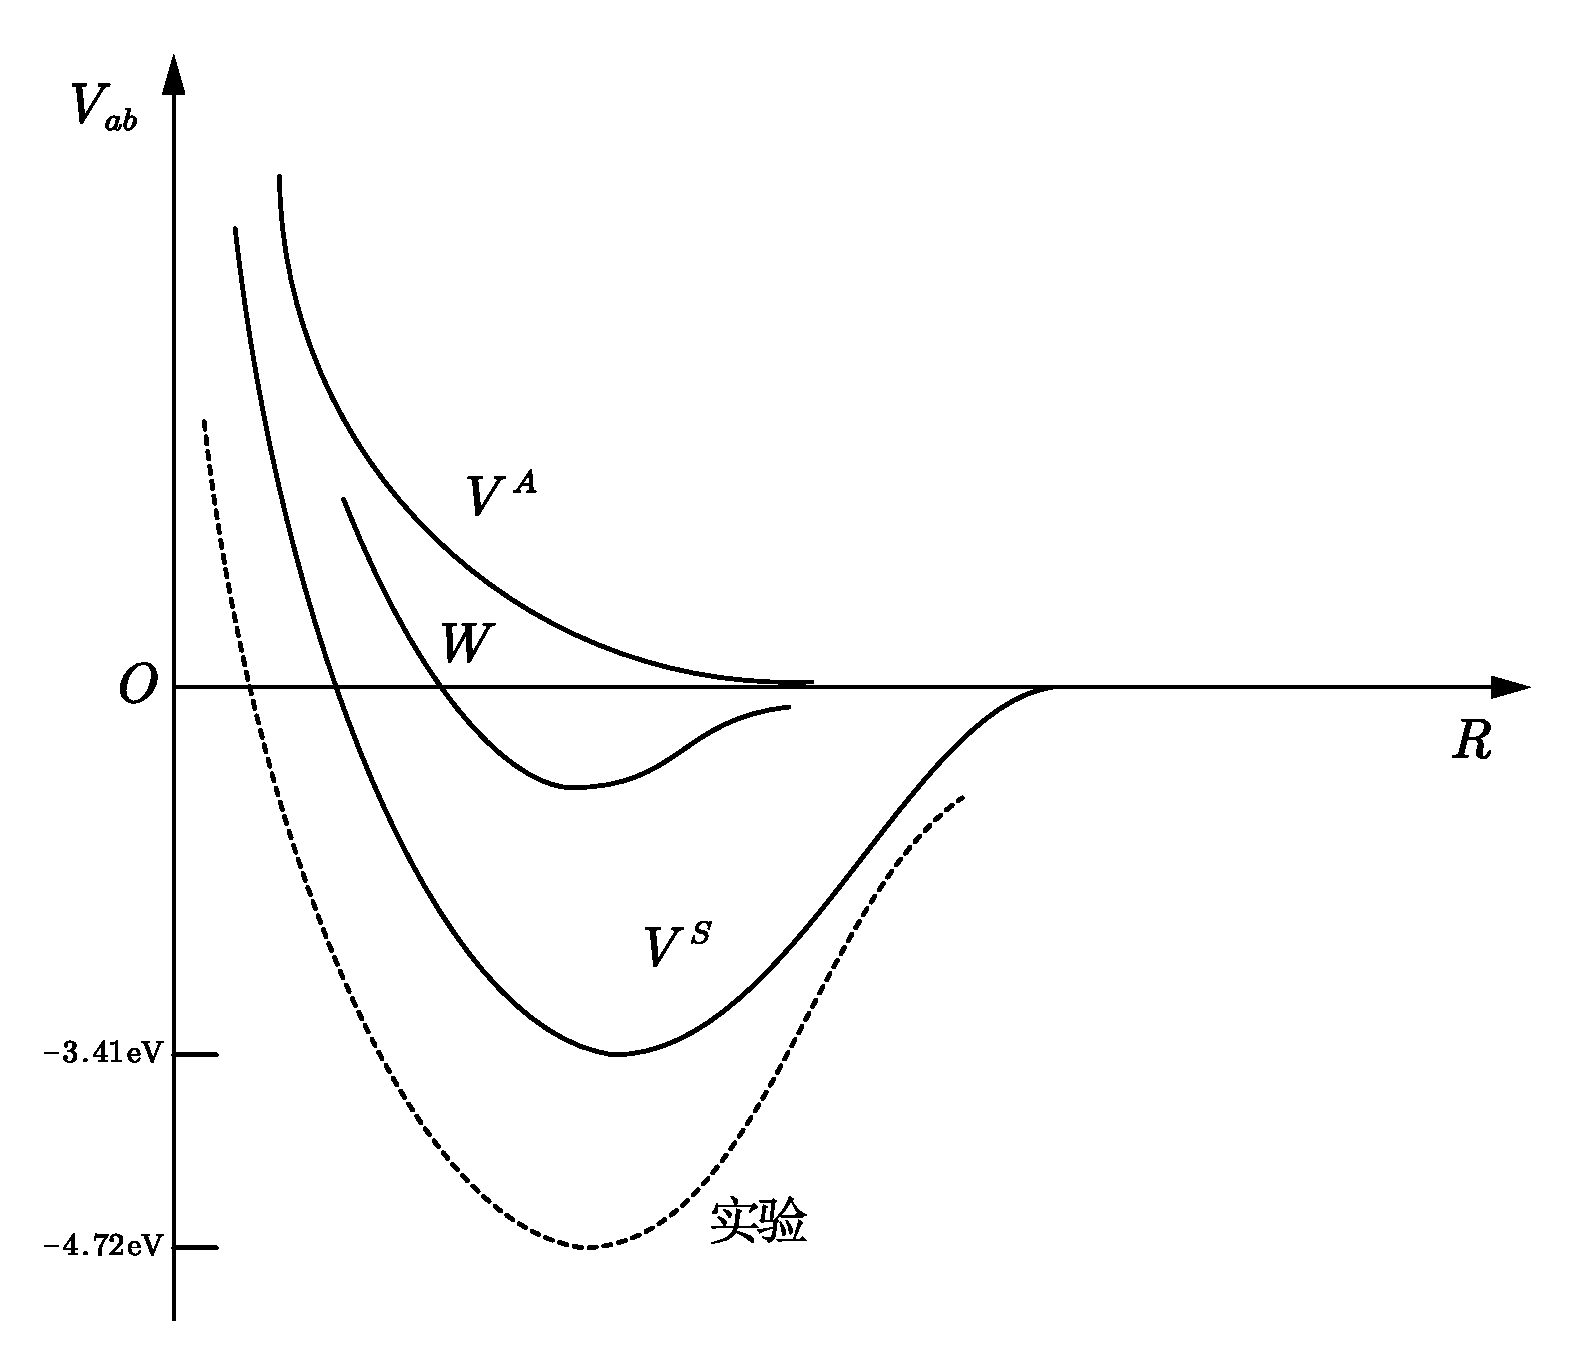
\includegraphics[width=5.5cm,clip]{QM file/figure/10-5}
	\caption{}\label{fig.10-5}
\end{figure}
\begin{wrapfigure}[7]{r}{7em}
	\centering
	\small
	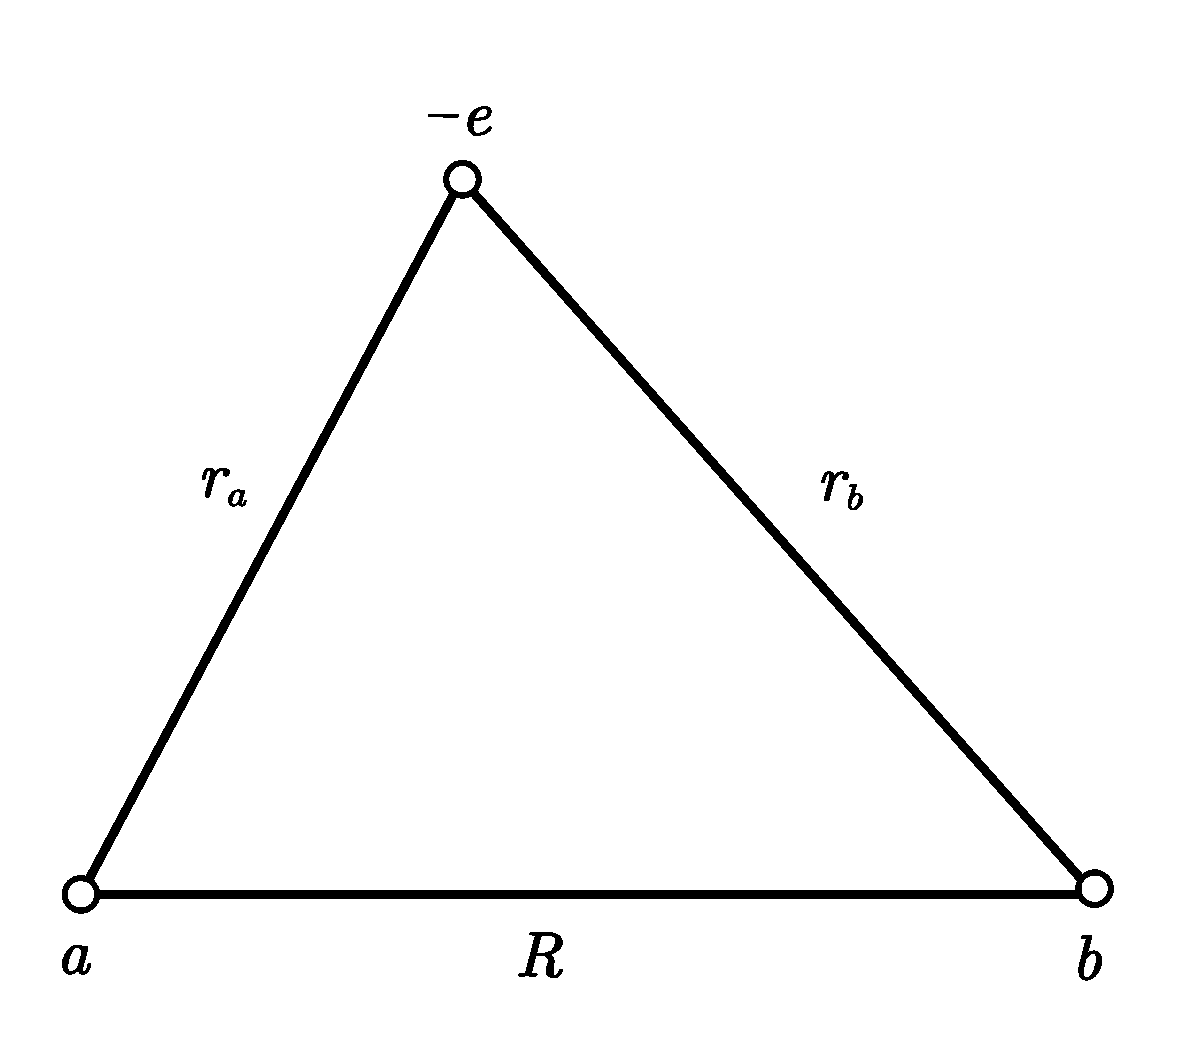
\includegraphics[width=3cm,clip]{QM file/figure/10-6}
	\caption{}\label{fig.10-6}
\end{wrapfigure}
詹姆斯等在考虑交换对称性的前提下,用变分法计算氢分子结合能.他们采用十分复杂的(包含13个变分参数)试探波函数,终于算出与实验值完全一致的结合能.

这表明分子的构造完全受量子力学规律支配,并没有任何超物理的因素起作用.

附录:重叠积分$D$和“库仑能”$W$的计算.

重叠积分$D$的定义见\eqref{eqx4.12}式,略去下标1,$D$可以写成
\begin{empheq}{equation*}
	D=\frac{1}{\pi a_{0}^{3}}\int e^{-(r_{a}+r_{b})/a_{0}}d\tau
\end{empheq}
$r_{a}$及$r_{b}$为电子至核$a$及核$b$之距离,如图10-6所示.引入共焦椭球坐标$(\xi,\eta,\varphi)$,定义为:
\begin{empheq}{align}\label{eqx4.17}
	\xi &=\frac{1}{R}(r_{a}+r_{b}),\quad 1\leqslant\xi <\infty	\\
	\eta&=\frac{1}{R}(r_{a}-r_{b}),\quad -1\leqslant\eta\leqslant1	\nonumber\\
	\varphi&\text{为绕ab轴的旋转角},0\leqslant\varphi <2\pi	\nonumber
\end{empheq}
体积元$d\tau$可以表示成
\begin{empheq}{equation}\label{eqx4.18}
	d\tau=\frac{R^{3}}{8}(\xi^{2}-\eta^{2})d\xi d\eta d\varphi
\end{empheq}
$r_{a},r_{b}$可以表示成
\begin{empheq}{equation}\label{eqx4.19}
	r_{a}=\frac{R}{2}(\xi+\eta),\quad r_{b}=\frac{R}{2}(\xi-\eta)
\end{empheq}\eqindent{5}
代入$D$中,即可算出
\begin{empheq}{align}\label{eqx4.20}
	D 
	&=\frac{1}{8\pi}\left(\frac{R}{a_{0}}\right)^{3}\int_{0}^{2\pi}d\varphi\int_{1}^{\infty}d\xi\int_{-1}^{1}d\eta(\xi^{2}-\eta^{2})e^{-\xi R/a_{0}}	\nonumber\\
	&=\frac{1}{4}\left(\frac{R}{a_{0}}\right)^{3}\int_{1}^{\infty}(2\xi^{2}-\frac{2}{3})e^{-\xi R/a_{0}}d\xi	\nonumber\\
	&=\left(1+\frac{R}{a_{0}}+\frac{1}{3}\frac{R^{2}}{a_{0}^{2}}\right)e^{-R/a_{0}}=D(R,a_{0})
\end{empheq}\eqnormal
此即\eqref{eqx4.12}式.积分的最后一步可用分部积分法算出.

“库仑能”$W$的定义见\eqref{eqx4.7}式.由于$\varPsi_{a}(1),\varPsi_{b}(2$均已归一化,显然
\begin{empheq}{equation*}
	\iint\varPsi_{a}^{2}(1)\varPsi_{b}^{2}(2)\frac{\e^{2}}{R}d\tau_{1}d\tau_{2}=\frac{\e^{2}}{R}
\end{empheq}\eqindent{5}
\begin{empheq}{align}\label{eqx4.21}
	&\iint\varPsi_{a}^{2}(1)\varPsi_{b}^{2}(2)\frac{1}{r_{1b}}d\tau_{1}d\tau_{2}
	=\iint\varPsi_{a}^{2}(1)\varPsi_{b}^{2}(2)\frac{1}{r_{2a}}d\tau_{1}d\tau_{2}	\nonumber\\
	&=\int\varPsi_{b}^{2}(2)\frac{1}{r_{2a}}d\tau_{2}=\frac{1}{\pi a_{0}^{3}}\int\frac{1}{r_{a}}e^{-2r_{b}/a_{0}}d\tau	\nonumber\\
	&=\frac{R^{3}}{4\pi a_{0}^{3}}\iiint d\xi d\eta d\varphi(\xi-\eta)e^{-(\xi-\eta)R/a_{0}}	\nonumber\\
	&=\frac{1}{R}-\left(\frac{1}{R}+\frac{1}{a_{0}}\right)e^{-2R/a_{0}}=I_{1}
\end{empheq}\eqnormal
\eqref{eqx4.7}式中较难的积分是
\begin{empheq}{equation}\label{eqx4.22}
	I_{2}=\iint\varPsi_{a}^{2}(1)\varPsi_{b}^{2}(2)\frac{1}{r_{12}}d\tau_{1}d\tau_{2}
\end{empheq}
先对d$\tau_{1}$积分,用普通球坐标,以原子核$a$作为坐标原点,对角度的积分仿照$\S$\ref{sec:10.03}曾用过的方法,$\frac{1}{r_{12}}$的积分效果相当于$\frac{1}{r_{2a}}$(当$r_{1a}<r_{2a}$)或$\frac{1}{r_{1a}}$(当$r_{2a}<r_{1a}$),因此
\begin{empheq}{align*}
	&\int\varPsi_{a}^{2}(1)\frac{d\tau_{1}}{r_{12}}=\frac{1}{\pi a_{0}^{3}}\int\frac{d\tau_{1}}{r_{12}}e^{-2r_{1a}/a_{0}}	\nonumber\\
	=&\frac{4}{a_{0}^{3}}\left[\frac{1}{r_{2a}}\int_{0}^{r_{2a}}drr^{2}e^{-2r/a_{0}}+\int_{r_{2a}}^{\infty}drre^{-2r/a_{0}}\right]
\end{empheq}
用分部积分法不难算出这二个积分,代入$I_{2}$中,整理后,可得
\begin{empheq}{equation*}\label{eqx4.22'}
	I_{2}=I_{1}-\frac{1}{8a_{0}}D\left(R,\frac{a_{0}}{2}\right)-I_{3}	\tag{$10.4.22^{\prime}$}
\end{empheq}
$D\left(R,\frac{a_{0}}{2}\right)$表示\eqref{eqx4.20}式中$a_{0}\rightarrow\frac{a_{0}}{2}$.$I_{3}$是下列积分:
\begin{empheq}{align}\label{eqx4.23}
	I_{3} &=\frac{1}{\pi a_{0}^{3}}\int\frac{d\tau}{r_{a}}e^{-2(r_{a}+r_{b})/a_{0}}	\nonumber\\
	&=\frac{R^{2}}{4\pi a_{0}^{3}}\iiint d\xi d\eta d\varphi(\xi-\eta)e^{-2\xi R/a_{0}}	\nonumber\\
	&=\frac{1}{4}\left(\frac{1}{a_{0}}+\frac{2R}{a_{0}^{2}}\right)e^{-2R/a_{0}}
\end{empheq}\eqlong
代入\eqref{eqx4.22'}式,即得
\begin{empheq}{equation}\label{eqx4.24}
	I_{2}=\frac{1}{R}-\frac{1}{R}\left(1+\frac{11R}{8a_{0}}+\frac{3R^{2}}{4a_{0}^{2}}+\frac{R^{3}}{6a_{0}^{3}}\right)e^{-2R/a_{0}}
\end{empheq}\eqnormal
以上结果代入\eqref{eqx4.7}式,即得\eqref{eqx4.8}式.



% 化学键
\section[化学键]{化学键} \label{sec:10.05} % 
% \makebox[5em][s]{} % 短题目拉间距

分子或晶体中将原子结合在一起的力都来自带电粒子间的库仑作用力.(和自旋有关的作用如自旋轨道耦合作用是微不足道的)按照键的物理机制和表现形式,大致分为离子键,共价键,金属键等类型.

正、负离子由于库仑吸引力而结合,就形成离子键.这种键的性质大体上用经典物理(静电学)就可以解释.如$\ce{Na^{+}}\ce{Cl^{-}}$晶体就是典型离子键晶体.

在共价键分子(或晶体)中,由于电子波函数的交换对称性,价电子比较集中地出现在二原子之间,通过它们与原子(离子)间的库仑吸引力而起键合作用.氢分子就是典型的共价键分子.共价键的形成,电子波函数的交换对称性起关键作用,是典型的量子力学效应,没有经典物理解释.

金属键是能带电子在晶体中公有化,在整个晶体中流动而产生的键合作用,性质接近共价键.金属键的概念来自固体物理,现已逐渐应用于量子化学,用来解释某些有机分子(如苯)的结构.

本节主要讨论共价键.由于篇幅所限,只作初浅的定性介绍.

上节讨论的氢分子是共价键分子的简单实例.两个原子间形成共价键时,通常“交换能”是负的,而且其绝对值远大于“库仑能”,结果导致构成键的一对电子处于自旋单态(反对称态)和轨道对称态,即$\Psi(q_{1},q_{2})=\chi_{00}(S_{1z}S_{2z})\varPsi^{S}(\boldsymbol{r}_{1},\boldsymbol{r}_{2})$,当两个电子位贸接近$(\boldsymbol{r}_{1}\sim\boldsymbol{r}_{2})$并处于两原子之间时,$|{\varPsi^{S}}|^{2}$较大,因此可以认为这一对价电子是被两个原子共同占有,共价键的名称即由此而来.

\begin{wrapfigure}[9]{r}{8em}
	\centering
	\small
	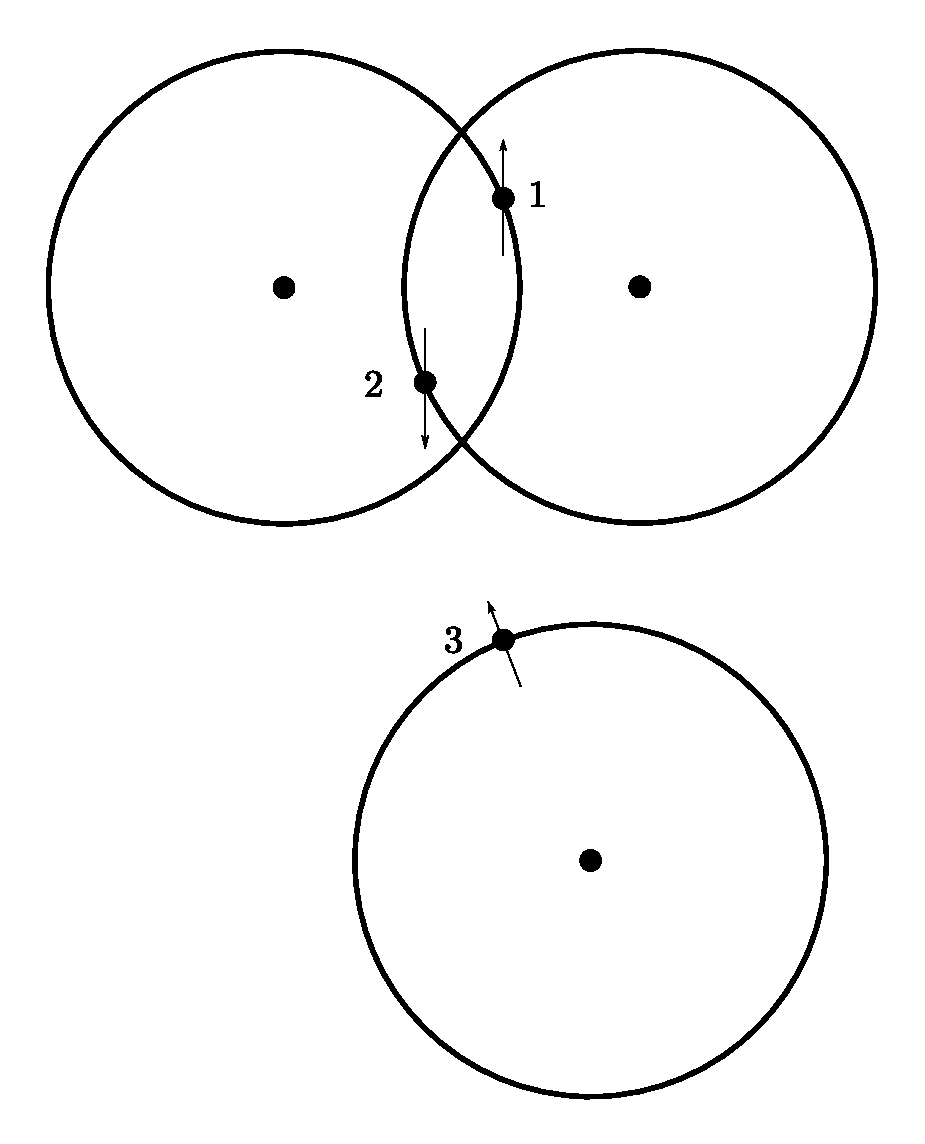
\includegraphics[width=2.5cm,clip]{QM file/figure/10-7}
	\caption{}\label{fig.10-7}
\end{wrapfigure}

共价键最显著的特点是饱和性.设想有第三个氢原子接近一个氢分子.后者的电子对已经处于自旋反对称态,两电子的自旋指向相反,总自旋为0.
外来的第三个电子已经不可能再与它们构成自旋反对称态,所以不能再形成键.从概率观点看问题,两个自旋指向混乱的电子(外来原子的电子与分子中的一个电子,参看图\ref{fig.10-7}),构成自旋对称态(三重态$\chi_{11},\chi_{10},\chi_{1-1}$)的概率是$\frac{3}{4}$,构成自旋反对称态(单态,$\chi_{00}$)的概率是$\frac{1}{4}$,而自旋对称态必为轨道反对称态,原子间的作用$(V^{A})$是排斥的结果是外来原子将受排斥.这就是共价键的饱和性.离子键就没有这种饱和性.

共价键的另一个特点是有方向性.共价键的形成是两个原子的价电子云重叠$(\boldsymbol{r}_{1}\sim\boldsymbol{r}_{2})$的结果,因此形成键的方向总是在价电子云的极大方向.氢原子中电子处于1s态,电子云分布各向同性,没有方向性,第二个原子可以从任何方向接近第一个原子而形成共价键,这种键没有方向性.如果原子的价电子是p态$(l=1)$或d态$(l=2)$电子,其电子云分布就有方向性.以p电子为例,共有3种独立轨道状态,即
\begin{empheq}{equation}\label{eqx5.1}
	\begin{aligned}
		&\varPsi_{npz}=\varPsi_{n10}=zF(r)	\\
	\varPsi_{npx}&=\frac{1}{\sqrt{2}}(\varPsi_{n1-1}-\varPsi_{n11})=xF(r)	\\
	\varPsi_{npy}&=\frac{i}{\sqrt{2}}(\varPsi_{n1-1}+\varPsi_{n11})=yF(r)
	\end{aligned}
\end{empheq}
电子云密度$\varPsi^{2}$的极大方向分别是$x,y,z$轴方向,如另一个原子的价电子(设为s电子)与这样的p电子构成共价键,键的方向必为p电子云的极大方向,如图\ref{fig.10-8}所示.

\begin{figure}[!h]
	\centering
	\small
	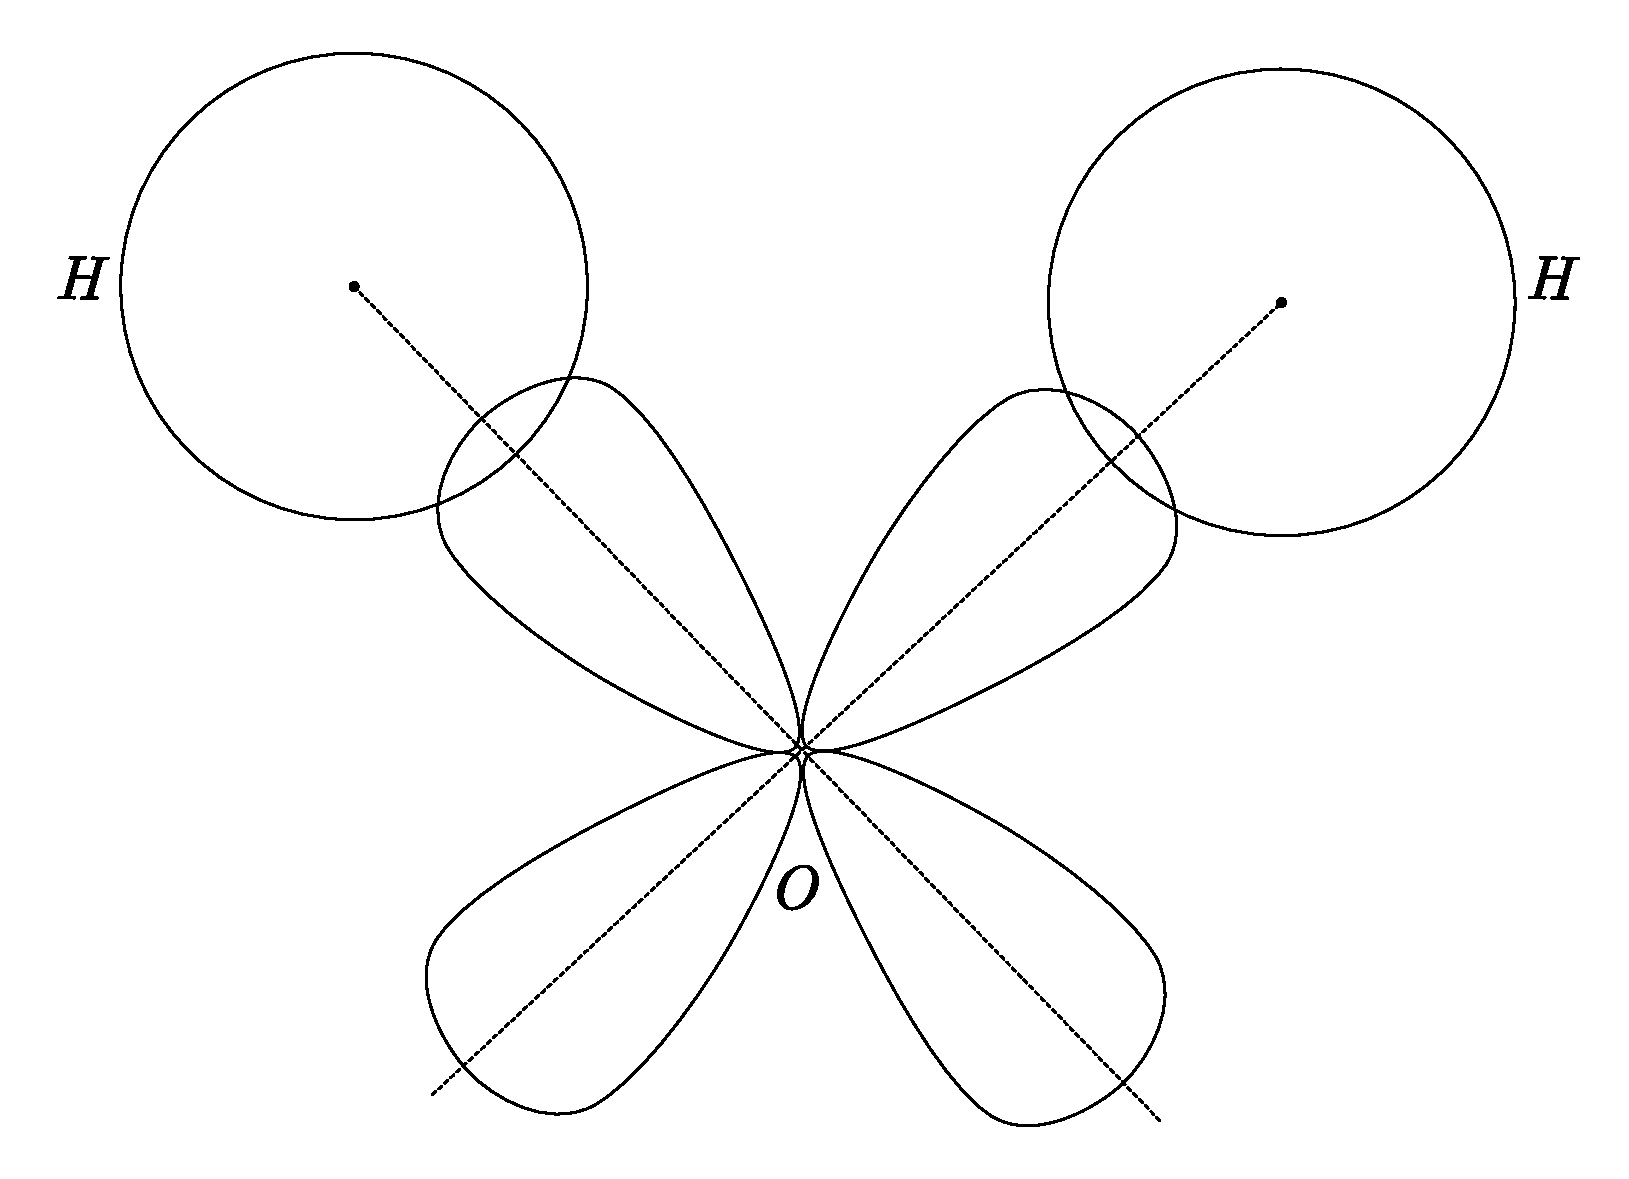
\includegraphics[width=7cm,clip]{QM file/figure/10-8}
	\caption{}\label{fig.10-8}
\end{figure}

以水$\ce{H_{2}O}$分子为例.氧原子中参与$\ce{H-O}$键的两个电子都是p电子,它们电子云的极大方向相互成$90^{\circ}$角.这两个p电子各自和一个氢原子的1s电子结合成共价键,如图\ref{fig.10-8}.由于$\ce{H-O}$键有少量离子键的因素(即$\ce{H^{+}-O^{--}-H^{+}}$),两个氢原子(离子)互相排斥,键角实际上增大成$105^{\circ}$.在19世纪,化学界曾想当然地以为$\ce{H_{2}O}$分子是直线式构造$\ce{H-O-H}$,有了量子化学,键的方向性概念以量子力学为理论依据,才被普遍承认.

在分子中,参与键的电子,由于受到邻近原子的影响,其原子状态严格地说已经与成键前不同.特别是,由于作用势的球对称性(各向同性)遭到破坏,价电子可以不再保持单一的$\boldsymbol{L}^{2}$本征值,其状态可以是s,p,d态的杂化态,这种处于杂化轨道的电子,其电子云分布更容易集中到某个方向,因此更有利于键的形成.量子化学利用杂化轨道理论成功地解释了许多分子构造问题.例如甲烷$(\ce{CH_{4}})$分子,碳$(\ce{C})$原子参与$\ce{C-H}$键的4个电子,本来的原子轨道是$(\ce{2s})^{2}(\ce{2p})^{2}$,由于轨道杂化,它们的单电子轨道态变成如下形式,
\begin{empheq}{equation}\label{eqx5.2}
	\varPsi(\boldsymbol{r})=a\varPsi_{\ce{2s}}+b\varPsi_{\ce{px}}+c\varPsi_{\ce{2py}}+d\varPsi_{\ce{2pz}}
\end{empheq}
当$(a,b,c,d)$取$(1,1,1,1)$,$(1,1,-1,-1)$,$(1,-1,1,-1)$,$(1,-1,-1,1)$时,电子云极大方向刚好是从正四面体中心指向4个顶点的方向,氢原子从这些方向接近,就容易结合成$\ce{C-H}$键.所以$\ce{CH_{4}}$分子中,4个$\ce{H}$原子正好处于正四面体顶点的位置,而$\ce{C}$原子处于对称中心.

半个多世纪以来,由于计算技术的进步和广泛运用量子力学理论及近似方法,量子化学已经发展成一门卓有成效的学科.




% 双原子分子的振动和转动
\starthis\section[双原子分子的振动和转动]{双原子分子的振动和转动} \label{sec:10.06} % 
% \makebox[5em][s]{} % 短题目拉间距

双原子分子的运动包括分子整体平移,转动,振动以及电子在定态能级上的运动和跃迁.如取分子质心坐标系,平移不必考虑电子能级(这里指价电子能级)的量级为10\si{eV}左右,分子振动能级的量级为$0.1\sim 1$\si{eV},转动能级约$10^{-3}\sim 10^{-4}$\si{eV}.例如氧分子$(\ce{O_{2}})$,实验数据为
\eqindent{8}

\begin{empheq}{alignat*=2}
	\text{键长}\num{0.1207}\si{nm}, &\qquad \text{离解能}\num{5.08}\si{eV} 	\\
	\hbar\omega=\num{0.196}\si{eV}, & \qquad \frac{\hbar^{2}}{2I}=\num{1.792}\times10^{-4}\si{eV}	\\
\end{empheq}\eqnormal
研究分子振动和转动时,电子能级一般不会变化,可以将原子当作一个内部结构不变的粒子,两个原子之间的作用以中心作用势$V(r)$表示($r$为两个原子的相对距离),$V-r$关系大体如$\S$\ref{sec:10.04}图\ref{fig.10-5}$\quad V^{5}-R$关系.

在分子质心坐标系中,分子的振动和转动即两原子的相对运动,等效于质量为$\mu$(折合质量)的粒子在中心势场$V(r)$中的运动,(参看$\S$\ref{sec:10.01})这个等效粒子的能量算符为
\begin{empheq}{equation}\label{eqx6.1}
	H=-\frac{\hbar^{2}}{2\mu}\nabla^{2}+V(r)
\end{empheq}
$V(r)$即两个原子间借以结合成分子的作用势,相当于$\S$\ref{sec:10.04}图\ref{fig.10-5}中的$V^{5}$.\eqref{eqx6.1}式中$(-i\hbar)\nabla$即二原子体系的相对动量$(\boldsymbol{p})$算符.相对角动量$\boldsymbol{L}=\boldsymbol{r}\times\boldsymbol{p}=-i\hbar\boldsymbol{r}\times\nabla$也就是分子的轨道角动量$(\boldsymbol{L}_{c}=0)$.$H,\boldsymbol{L}^{2},L_{z}$的共同本征函数可以表示成(参看$\S$\ref{sec:05.01})
\begin{empheq}{equation}\label{eqx6.2}
	\varPsi=R(r)Y_{lm}(\theta,\varphi)=\frac{1}{r}u(r)Y_{lm}(\theta,\varphi)
\end{empheq}
其中球谐函数$Y_{lm}$描写分子转动.$u(r)$满足径向方程
\begin{empheq}{equation}\label{eqx6.3}
	-\frac{\hbar^{2}}{2\mu}\frac{d^{2}}{dr^{2}}u+\left[V(r)+\frac{l(l+1)\hbar^{2}}{2\mu r^{2}}\right]u=Eu
\end{empheq}
$u(r)$描述相对径向运动,即振动.$E$为总能量,即振动,转动能量的总和再加上分子结合能[下面\eqref{eqx6.4}式中$V_{0}$.]

设分子键长为$R$,则$r=R$处$V(r)$为极小.如振动的振幅很小,即$|r-R\ll R$,可将$V(r)$展开成$(r-R)$的幕级数而略去$(r-R)^{3}$以上各项,取
\begin{empheq}{align}\label{eqx6.4}
	V(r)&=V_{0}+\frac{1}{2}V^{\prime\prime}(R)(r-R)^{2}	\nonumber\\
	&=V_{0}+\frac{1}{2}\mu\omega_{0}^{2}(r-R)^{2}
\end{empheq}
$V_{0}$即$V(R)$.将\eqref{eqx6.4}式代入\eqref{eqx6.3}式,得到
\begin{empheq}{align}
	-\frac{\hbar^{2}}{2\mu}\frac{d^{2}}{dr^{2}}u+V_{l}(r)u=(E-V_{0})u	\label{eqx6.5}\\
	V_{l}(r)=\frac{1}{2}\mu\omega_{0}^{2}(r-R)^{2}+\frac{l(l+1)\hbar^{2}}{2\mu r^{2}}	\label{eqx6.6}
\end{empheq}
$(E-V_{0})$为振动与转动能量之和,$V_{l}(r)$是等效势能.当$r=R$,$V_{l}$中第二项(离心势能)即通常所说分子转动能级,记为$E_{l}$
\begin{empheq}{equation}\label{eqx6.7}
	E_{l}=\frac{l(l+1)\hbar^{2}}{2\mu R^{2}}=\frac{l(l+1)\hbar^{2}}{2I}
\end{empheq}\eqshort
$I=\mu R^{2}$为分子转动惯量.设
\begin{empheq}{equation}\label{eqx6.8}
	E_{l}\ll \frac{1}{2}\mu\omega_{0}^{2}R^{2}
\end{empheq}\eqnormal
(上式右端相当于振动的振幅等于键长$R$时的振动能,这样大的能量足以使分子离解.所以上式总是成立的.)在这条件下$V_{l}$将存在极小,其位置可由极值条件$\frac{dV_{l}}{dr}=0$来确定,如下.
\begin{empheq}{align}\label{eqx6.9}
	\frac{d}{dr}V_{l}(r) &=\mu\omega_{0}^{2}(r-R)-\frac{l(l+1)\hbar^{2}}{\mu r^{3}}	\nonumber\\
	&\approx\mu\omega_{0}^{2}(r-R)-\frac{l(l+1)\hbar^{2}}{\mu R^{3}}=0	\nonumber\\
	r&=R+\frac{l(l+1)\hbar^{2}}{\mu^{2}\omega_{0}^{2}R^{3}}\xlongequal{\text{令}}r_{0}
\end{empheq}
如将$R$看成分子的静态(振动、转动完全消失)键长,则$r_{0}$就是动态键长,其中第二项是由于转动而引起的键的伸长.将$V_{l}(r)$在$r_{0}$附近展开成$(r-r_{0})$的幕级数,略去$(r-r_{0})^{3}$以上各项,得到
\begin{empheq}{equation}\label{eqx6.10}
	V_{l}(r)=V_{l}(r_{0})+\frac{1}{2}V_{l}^{\prime\prime}(r_{0})(r-r_{0})^{2}
\end{empheq}
如令
\begin{empheq}{equation}\label{eqx6.11}
	x=r-r_{0},\quad V_{l}^{\prime\prime}=\mu\omega_{0}^{2}
\end{empheq}
即得
\begin{empheq}{equation*}\label{eqx6.10'}
	V_{l}(r)=V_{l}(r_{0})+\frac{1}{2}\mu\omega_{0}^{2}x^{2}
	\tag{$10.6.10^{\prime}$}
\end{empheq}\eqlong
代入径向方程\eqref{eqx6.5}式,成为
\begin{empheq}{equation}\label{eqx6.12}
	-\frac{\hbar^{2}}{2\mu}\frac{d^{2}}{dx^{2}}+\frac{1}{2}\mu\omega^{2}u=[E-V_{0}-V_{l}(r_{0})]u=E^{\prime}u
\end{empheq}\eqllong
上式形式上和一维谐振子的能量本征方程相同,利用谐振子能级公式,即可得出
\begin{empheq}{equation}\label{eqx6.13}
	E-V_{0}-V_{l}(r_{0})=E^{\prime}=\left(\nu+\frac{1}{2}\right)\hbar\omega,\quad \nu=0,1,2,\cdots
\end{empheq}\eqlong
$\nu$为振动量子数.由\eqref{eqx6.6}、\eqref{eqx6.9}式容易求出
\begin{empheq}{align}\label{eqx6.14}
	V_{l}(r_{0}) &=\frac{1}{2}\mu\omega_{0}^{2}\left[\frac{l(l+1)\hbar^{2}}{\mu^{2}\omega_{0}^{2}R^{3}}\right]+\frac{l(l+1)\hbar^{2}}{2\mu r_{0}^{2}}	\nonumber\\
	&\approx E_{l}-\frac{l^{2}(l+1)^{2}\hbar^{4}}{2\mu^{2}\omega_{0}^{2}R^{6}}
\end{empheq}\eqindent{11}
计算中作了近似处理
\begin{empheq}{equation*}
	\frac{1}{r_{0}^{2}}\approx\frac{1}{R^{2}}-\frac{2l(l+1)\hbar^{2}}{\mu^{2}\omega_{0}^{2}R^{6}}
\end{empheq}
由\eqref{eqx6.6}、\eqref{eqx6.9}、\eqref{eqx6.11}式可以求出
\begin{empheq}{align}\label{eqx6.15}
	\omega^{2} &=\omega_{0}^{2}+\frac{3l(l+1)\hbar^{2}}{\mu^{2}r_{0}^{4}} \nonumber\\
	\omega&\approx\omega_{0}+\frac{3l(l+1)\hbar^{2}}{2\mu^{2}\omega_{0}R^{4}}
\end{empheq}\eqnormal
其中第二项是由于转动而引起的振动频率变化.将以上结果代入\eqref{eqx6.13}式,即得分子振-转能级的最后表达式
\begin{empheq}{equation}\label{eqx6.16}
	\begin{aligned}
	E_{\nu l}&=E-V_{0}=V_{l}(r_{0})+\left(\nu+\frac{1}{2}\right)\hbar\omega	\\
	&\approx\left(\nu+\frac{1}{2}\right)\hbar\omega+E_{l}-\frac{l^{2}(l+1)^{2}\hbar^{4}}{2\mu^{2}\omega_{0}^{2}R^{6}}	\\
	E_{l}&=\frac{l(l+1)\hbar^{2}}{2\mu R^{2}},\quad l,\nu=0,1,2,\cdots
	\end{aligned}
\end{empheq}
$E_{l}$即上述转动能级,$\left(\nu+\frac{1}{2}\right)\hbar\omega$常称为振动能级,$E_{\nu l}$中最后一项则是由于键长改变而产生的能级修正,称为振-转修正项.


% 习题
\begin{exercises}

\exercise 两个质量为$m$的全同粒子,在一维弹性力场中运动,$V_{1}=\dfrac{kx_{1}^{2}}{2},V_{2}=\dfrac{kx_{2}^{2}}{2}$,两粒子间的相互作用可以忽略.

(a) 写出体系的总能量算符,分别用$(x_{1},x_{2})$表示和$(X,x)$表示.($X$是质心坐标,$x$是相对坐标)讨论质心运动和相对运动的性质.

(b) 写出单粒子运动的基态与第一激发态波函数.($\varPsi_{0}$与$\varPsi_{1}$,略去归一化常数)如一个粒子处于基态,一个粒子处于第一激发态,写出对称的和反对称的体系轨道波函数,先用$(x_{1},x_{2})$表示,再用$(X,x)$表示,解释其性质.
\pskip
\exercise 两个质量为$m$的非全同粒子,受到外场作用,还有相互作用,作用势为
\eqllong
\begin{empheq}{equation*}
	V_{1}=\frac{\alpha}{2}x_{1}^{2},\quad V_{2}=\frac{\alpha}{2}x_{2}^{2},\quad V_{12}=\frac{\beta}{2}(x_{1}^{2}-x_{2}^{2})\quad (\alpha,\beta>0)
\end{empheq}\eqnormal

求体系的能谱.
\pskip
\exercise 某体系由3个自旋为0的全同粒子组成,限定单粒子状态只能是$\varPsi_{\alpha},\varPsi_{\beta},\varPsi_{\gamma}$,试写出体系的所有可能状态的波函数.

\exercise 两个自旋为0的全同粒子在无限深势阱$(0<x_{i}<a,i=1,2)$中运动,忽略粒子间相互作用.写出这个二粒子体系的基态与第一激发态波函数,并对基态计算$\bar{x},\Delta x,\bar{X},\Delta X$.

[提示:先计算$\bar{x_{1}},\bar{x_{2}},\bar{x_{1}^{2}},\bar{x_{2}^{2}}$.]
\pskip
\exercise 两个质量相同的粒子在无限深势阱$(0<x_{i}<a,i=1,2)$中运动.粒子间相互作用势$V_{12}=aV_{0}\delta(x_{1}-x_{2}),V_{0}\ll\dfrac{\hbar^{2}}{ma^{2}}$,因此可以视之为微扰.求这二粒子体系最低的3个能级.(不考虑粒子是否全同.)
\pskip
\exercise 类氦离子由原子核(电荷$Ze,Z>2$)及两个电子构成.如略去核运动,二电子体系总能量算符可以写成
\begin{empheq}{equation*}
	H=-\frac{\hbar^{2}}{2m_{e}}(\nabla_{1}^{2}+\nabla_{2}^{2})-Z\e^{2}\left(\frac{1}{r_{1}}+\frac{1}{r_{2}}\right)+\frac{\e^{2}}{r_{12}}
\end{empheq}\eqllong

(a) 视$\dfrac{\e^{2}}{r_{12}}$为微扰,求基态能级的粗略近似.

(b) 用变分法求基态能级近似值.
\pskip
\exercise 有-种简化的“一维类氦离子”模型,原子核-电子和电子-电子作用势均用“接触作用”表示.略去核运动后,电子体系总能量算符表示成
\begin{empheq}{equation*}
	H=-\frac{\hbar^{2}}{2m_{e}}\left(\frac{\partial^{2}}{\partial x_{1}^{2}}+\frac{\partial^{2}}{\partial x_{2}^{2}}\right)-Z\e^{2}[\delta(x_{1})+\delta(x_{2})]+\e^{2}\delta(x_{1}-x_{2})
\end{empheq}\eqlong

如距离以$\dfrac{a_{0}}{Z}$为单位,能量以$\dfrac{Z^{2}\e^{2}}{a_{0}}$为单位,$H$可以简化成
\begin{empheq}{equation*}
	H=-\frac{1}{2}\left(\frac{\partial^{2}}{\partial x_{1}^{2}}+\frac{\partial^{2}}{\partial x_{2}^{2}}\right)-\delta(x_{1})-\delta(x_{2})+\frac{1}{Z}\delta(x_{1}-x_{2})
\end{empheq}

(a) 视电子-电子作用势为微扰,求体系束缚态能级(只有一个).

(b) 用变分法求体系能级.

你将发现本题结果与10-6题结果惊人地接近.
\pskip
\exercise 某个三电子体系,单电子轨道态为$\varPsi_{a},\varPsi_{b},\varPsi_{c}$.当体系总自旋量子数$S=\dfrac{3}{2}$时,写出体系的轨道波函数,求相互作用能$\left(\dfrac{\e^{2}}{r_{12}}+\dfrac{\e^{2}}{r_{23}}+\dfrac{\e^{2}}{r_{31}}\text{的平均值}\right)$,将其表示成“库仑能”和“交换能”.
\pskip
\exercise 由两个全同粒子组成的体系,如单粒子自旋量子数为S,$[\boldsymbol{S}^{2}=S(S+1)\hbar^{2}]$体系总自旋态有多少种独立的交换对称态、反对称态?
\pskip
\exercise (a) 如原子中的电子换成某种电荷为$(-e)$,自旋量子数为$\dfrac{3}{2}$的粒子,求前三种惰性气体的原子序数($Z$,核中质子数)

(b) 如原子中的电子换成某种电荷为$(-\dfrac{e}{3})$,自旋量子数为$\dfrac{1}{2}$的费密子,求前三种惰性气体的原子序数.
\pskip
\exercise 两电子体系,定义“自旋交换算符”$P_{12},P_{12}\chi(S_{1z},S_{2z})=\chi(S_{2z},S_{1z})$,证明:$P_{12}=\dfrac{1}{2}(1+\boldsymbol{\sigma}_{1}\cdot\boldsymbol{\sigma}_{2})=\boldsymbol{S}^{2}-1$.($\boldsymbol{S}$为总自旋,取$\hbar=1$)
\pskip
\exercise 设粒子1,2自旋量子数均为$\dfrac{1}{2}$,以$\boldsymbol{S}=\boldsymbol{S}_{1}+\boldsymbol{S}_{2}$表示总自旋算符,取$\hbar=1$.证明以下算符关系:

\begin{empheq}{alignat*=2}
	[\boldsymbol{S}_{1}\cdot\boldsymbol{S}_{2},\boldsymbol{S}_{1}]=i\boldsymbol{S}_{1}\times\boldsymbol{S}_{2}, &\quad [\boldsymbol{S}_{1}\cdot\boldsymbol{S}_{2},\boldsymbol{S}_{2}]=-i\boldsymbol{S}_{1}\times\boldsymbol{S}_{2}	\\
	[\boldsymbol{S}_{1}\cdot\boldsymbol{S}_{2},\boldsymbol{S}]=0, &\quad  \boldsymbol{S}\boldsymbol{S}^{2}=\boldsymbol{S}^{2}\boldsymbol{S}=2\boldsymbol{S}	\\
\end{empheq}\eqnormal

\exercise 两个自旋量子数为$\dfrac{1}{2}$的非全同粒子,位置固定,相互作用能(算符)为$H=\dfrac{\omega}{\hbar}\boldsymbol{S}_{1}\cdot\boldsymbol{S}_{2}$时粒子1自旋$(\boldsymbol{S}_{1})$沿正$z$轴方向极化,粒子2自旋$(\boldsymbol{S}_{2})$极化方向正好相反.对于任意$t>0$时刻,

(a) 求体系总自旋波函数$\chi(t)$,用单粒子自旋态$\alpha(1),\beta(1),\alpha(2),\beta(2)$表示出来,[提示:将初始总自旋态展开成$H$的本征态的叠加.]

(b) 求$\boldsymbol{S}_{1}$极化方向与初始指向相同的概率.

(c) 求$\boldsymbol{S}_{1}$和$\boldsymbol{S}_{2}$极化方向均指向正$z$轴的概率.

(d) 总自旋量子数$S=1,0$的各自概率.
\pskip
\exercise 如原子的最外层是两个单粒子能级为$E_{nl}$的电子,作为二电子体系,讨论其总$L,S,J$的可能取值组合,证明$L+S=$偶数.

[提示:注意波函数的交换对称性,同时参看$\S$\ref{sec:10.02}例题.]
\pskip
\exercise 已知氘核(d)自旋为$\hbar$,宇称为偶;中子(n)自旋为$\dfrac{\hbar}{2}$;$\pi^{-}$介子自旋为0.试根据反应
\begin{empheq}{equation*}
	\pi^{-}\text{(静止)}+\ce{d}\rightarrow \ce{n}+\ce{n}
\end{empheq}

决定$\pi^{-}$介子的内禀宇称.

[提示:反应前后角动量守恒,宇称守恒.反应后为费密子体系.]
\pskip
\exercise 考虑一个多电子原子或分子,总能量包括各个电子及原子核的动能以及粒子间的库仑势能.(忽略自旋和相对论效应)体系的基态能级记为$E_{0}$,基态波函数记为$\varPsi_{0}$,预备用变分法找$E_{0}$,$\varPsi_{0}$的近似.设己找到$\varPsi_{0}$的粗略近似$\phi(\boldsymbol{r}_{1},\boldsymbol{r}_{2},\cdots,\boldsymbol{r}_{N})$,并已求出体系动能平均值$W$,势能平均值$U<0$,再取试探波函数为$\varPsi(\lambda)=\lambda^{\dfrac{3N}{2}}\phi(\lambda\boldsymbol{r}_{1},\cdots,\lambda\boldsymbol{r}_{N})$.证明:

(a) $\lambda$最佳值为$\lambda_{0}=-\dfrac{U}{2W}$,$E_{0}$近似值$E(\lambda_{0})=-\dfrac{U^{2}}{4W}$.

(b) 如$\phi(\boldsymbol{r}_{1},\cdots,\boldsymbol{r}_{N})$刚好就是$\varPsi_{0}$,则$U=-2W,E_{0}=W+U$(即位力定理结论)试将本题结论用于氦原子,利用微扰论结果直接得出变分法结果.

\end{exercises}
